%%%%%%%%%%%%%%%%%%%%%%%%%%%%%%%%%%%%%%%%%%%%%%%%%%%%%%%%%%%%%%%%%%%%%
% LaTeX Template: Project Titlepage Modified (v 0.1) by rcx
%
% Original Source: http://www.howtotex.com
% Date: February 2014
%
% This is a title page template which be used for articles & reports.
%
% This is the modified version of the original Latex template from
% aforementioned website.
%
%%%%%%%%%%%%%%%%%%%%%%%%%%%%%%%%%%%%%%%%%%%%%%%%%%%%%%%%%%%%%%%%%%%%%%

\documentclass[12pt]{report}
\usepackage[a4paper]{geometry}
\usepackage[myheadings]{fullpage}
\usepackage{fancyhdr}
\usepackage{lastpage}
\usepackage{graphicx, wrapfig, subcaption, setspace, booktabs}
\usepackage[T1]{fontenc}
\usepackage[font=small, labelfont=bf]{caption}
\usepackage{fourier}
\usepackage[protrusion=true, expansion=true]{microtype}
\usepackage[english]{babel}
\usepackage{sectsty}
\usepackage{url, lipsum}
\usepackage{multicol}


\newcommand{\HRule}[1]{\rule{\linewidth}{#1}}
\onehalfspacing
\setcounter{tocdepth}{5}
\setcounter{secnumdepth}{0}

%-------------------------------------------------------------------------------
% HEADER & FOOTER
%-------------------------------------------------------------------------------
\pagestyle{fancy}
\fancyhf{}
\setlength\headheight{15pt}
\fancyhead[L]{Team 5}
\fancyhead[R]{AFRS Release 2}
\fancyfoot[R]{Page \thepage\ of \pageref{LastPage}}
%-------------------------------------------------------------------------------
% TITLE PAGE
%-------------------------------------------------------------------------------

\begin{document}

    \title{ \normalsize \textsc{SWEN 262}
    \\ [2.0cm]
    \HRule{0.5pt} \\
    \LARGE \textbf{\uppercase{AFRS Release 2}}
    \HRule{2pt} \\ [0.5cm]
    \normalsize \today \vspace*{5\baselineskip}}

    \date{}

    \author{
    Devin Matte drm8019@rit.edu \\
    Amanda Ramos alr7924@rit.edu \\
    Nicholas Montemorano nmm9422@rit.edu \\
    Oren Rosin oxr3231@rit.edu
    }

    \maketitle
    \tableofcontents
    \newpage

    %-------------------------------------------------------------------------------
    % Section title formatting
    \sectionfont{\scshape}
    %-------------------------------------------------------------------------------

    %-------------------------------------------------------------------------------
    % BODY
    %-------------------------------------------------------------------------------

    \section*{Summary}\label{sec:summary}
    \addcontentsline{toc}{section}{Summary}

    \indent
    The AFRS lets clients request reservations for flights.
    The system responds with the possible flight plans, giving the user the power to choose one.
    The system will ask the user for a command and said user can put a command in to make, delete or save a reservation for a passenger name.
    The system keeps track of all reservations and flight data.
    While in the terminal, the user can also input a code for an airport to view all information of the airport such as weather, delay times, flights and location.
    A user can also get date for each flight stored in the system.
    \newline
    \indent
    As of the most recent release, the user can no also undo a command recently performed, they can utilize a GUI interface, use data either from the local system or the FAA, as well as being able to have multiple concurrent clients.
    The system now allows for users across of Treetop Airways to enjoy a more simplistic and useful interface as they manage the reservations throughout the system.
    \newpage

    %-------------------------------------------------------------------------------
    % Release 2 Design Updates
    %-------------------------------------------------------------------------------
    \section*{Release 2 Design Updates}\label{sec:release2DesignUpdates}
    \addcontentsline{toc}{section}{Release 2 Design Updates}

    \indent
    Overall the system coming from release 1 was in a good state.
    The features and requirements from Release 1 were all implemented and functional to the standard.
    Now when it came to Release 2, there was a need for a break up between client and server interactions.
    This being that there now needs to be the ability for multiple concurrent clients all performing commands on the system.
    Because of this, there was a need to break the system out into a client/server/common layout.
    \newline
    \indent
    The main way to describe this breakout is that the client, cannot directly use any classes from the server, and the server vice versa.
    However there are parts of the system that both need to access, that should be called the common, which are common classes shared by both systems.
    \newline
    \indent
    This design required a bit of refactoring and an idea of how we could implement the communication between the clients and the server.
    The discussion landed on using a web route based web service as the server.
    This would allow the client to make simple http calls using a RESTful API to a constantly running server.

    \begin{center}
        \makebox[\textwidth]{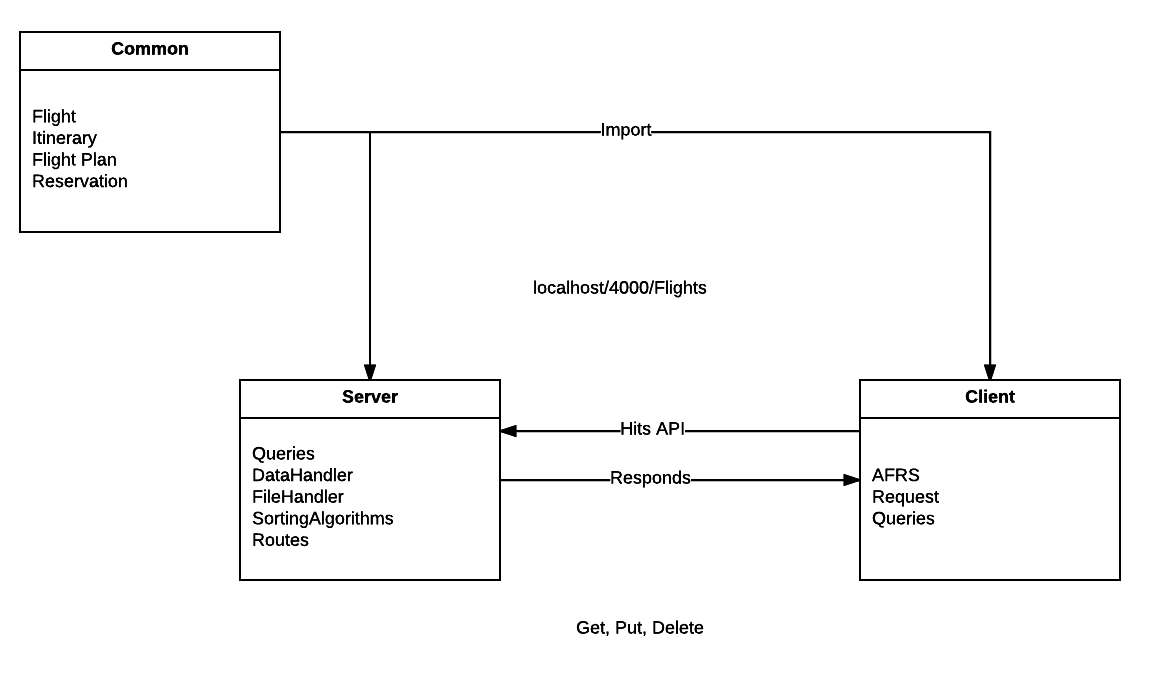
\includegraphics[width=\linewidth]{images/r2-refactor.png}}
    \end{center}

    \indent
    With this new design in mind, we then had to take into account our current subsystems and how they would fit into this new release, especially with the need to use a series of new design patterns from iterator, proxy and state patterns.
    State pattern seemed like an easy implementation with the use of FFA or Flat files being a state, and the use of the CMD interface vs the GUI being another.
    Proxy seemed like another easier implementation given the fact that the API is not called directly by the AFRS client, but instead is called through command pattern style classes, that then, by proxy, call the server.
    Iterator was a bit harder of a decision to make as to where it should be implemented.

    %-------------------------------------------------------------------------------
    % Domain Model
    %-------------------------------------------------------------------------------
    \newpage
    \section*{Domain Model}\label{sec:domainModel}
    \addcontentsline{toc}{section}{Domain Model}

    \paragraph{Release 1}

    \indent
    Release 1 Design was a little underdeveloped.
    There was a functional system, however it was not very well thought out in the overall design.
    There was a lot of work to be done on how the system communicated as a whole.
    In Release 1 the focus was on getting a system that worked, and worked in a logical way instead of on how to design a system that was easy to continue development on after the fact.
    Because of this the design made sense, but was not very thought out.

    \begin{center}
        \makebox[\textwidth]{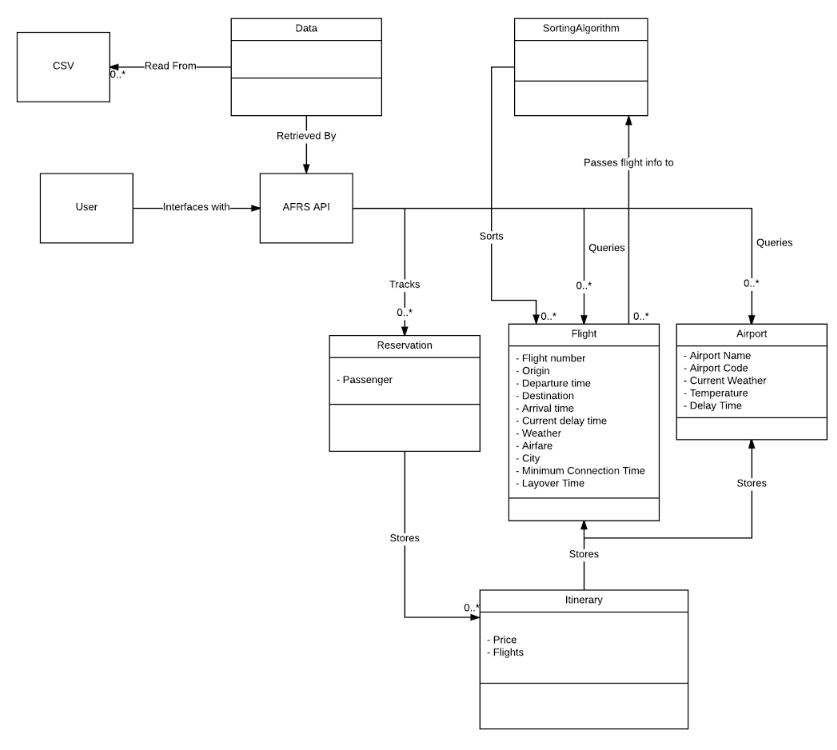
\includegraphics[width=\linewidth]{images/r1domainmodel.png}}
    \end{center}

    \paragraph{Release 2}

    \indent
    Release 2 we took the client/server/common design approach and found a decent amount of success doing so.
    The design when split into client and server made a lot of sense as to not only how communication works, but also how the system as a whole should be laid out.
    By splitting communication we also heavily decoupled the system.
    The client relies on the server, but the server has no reliance whatsoever on the client, and the client has a lot less information as it only knows what the user and the server give it.
    Before the client was responsible for all interactions with the datahandler, and the user.
    This creates a good layer of abstraction as well as decoupling.

    \begin{center}
        \makebox[\textwidth]{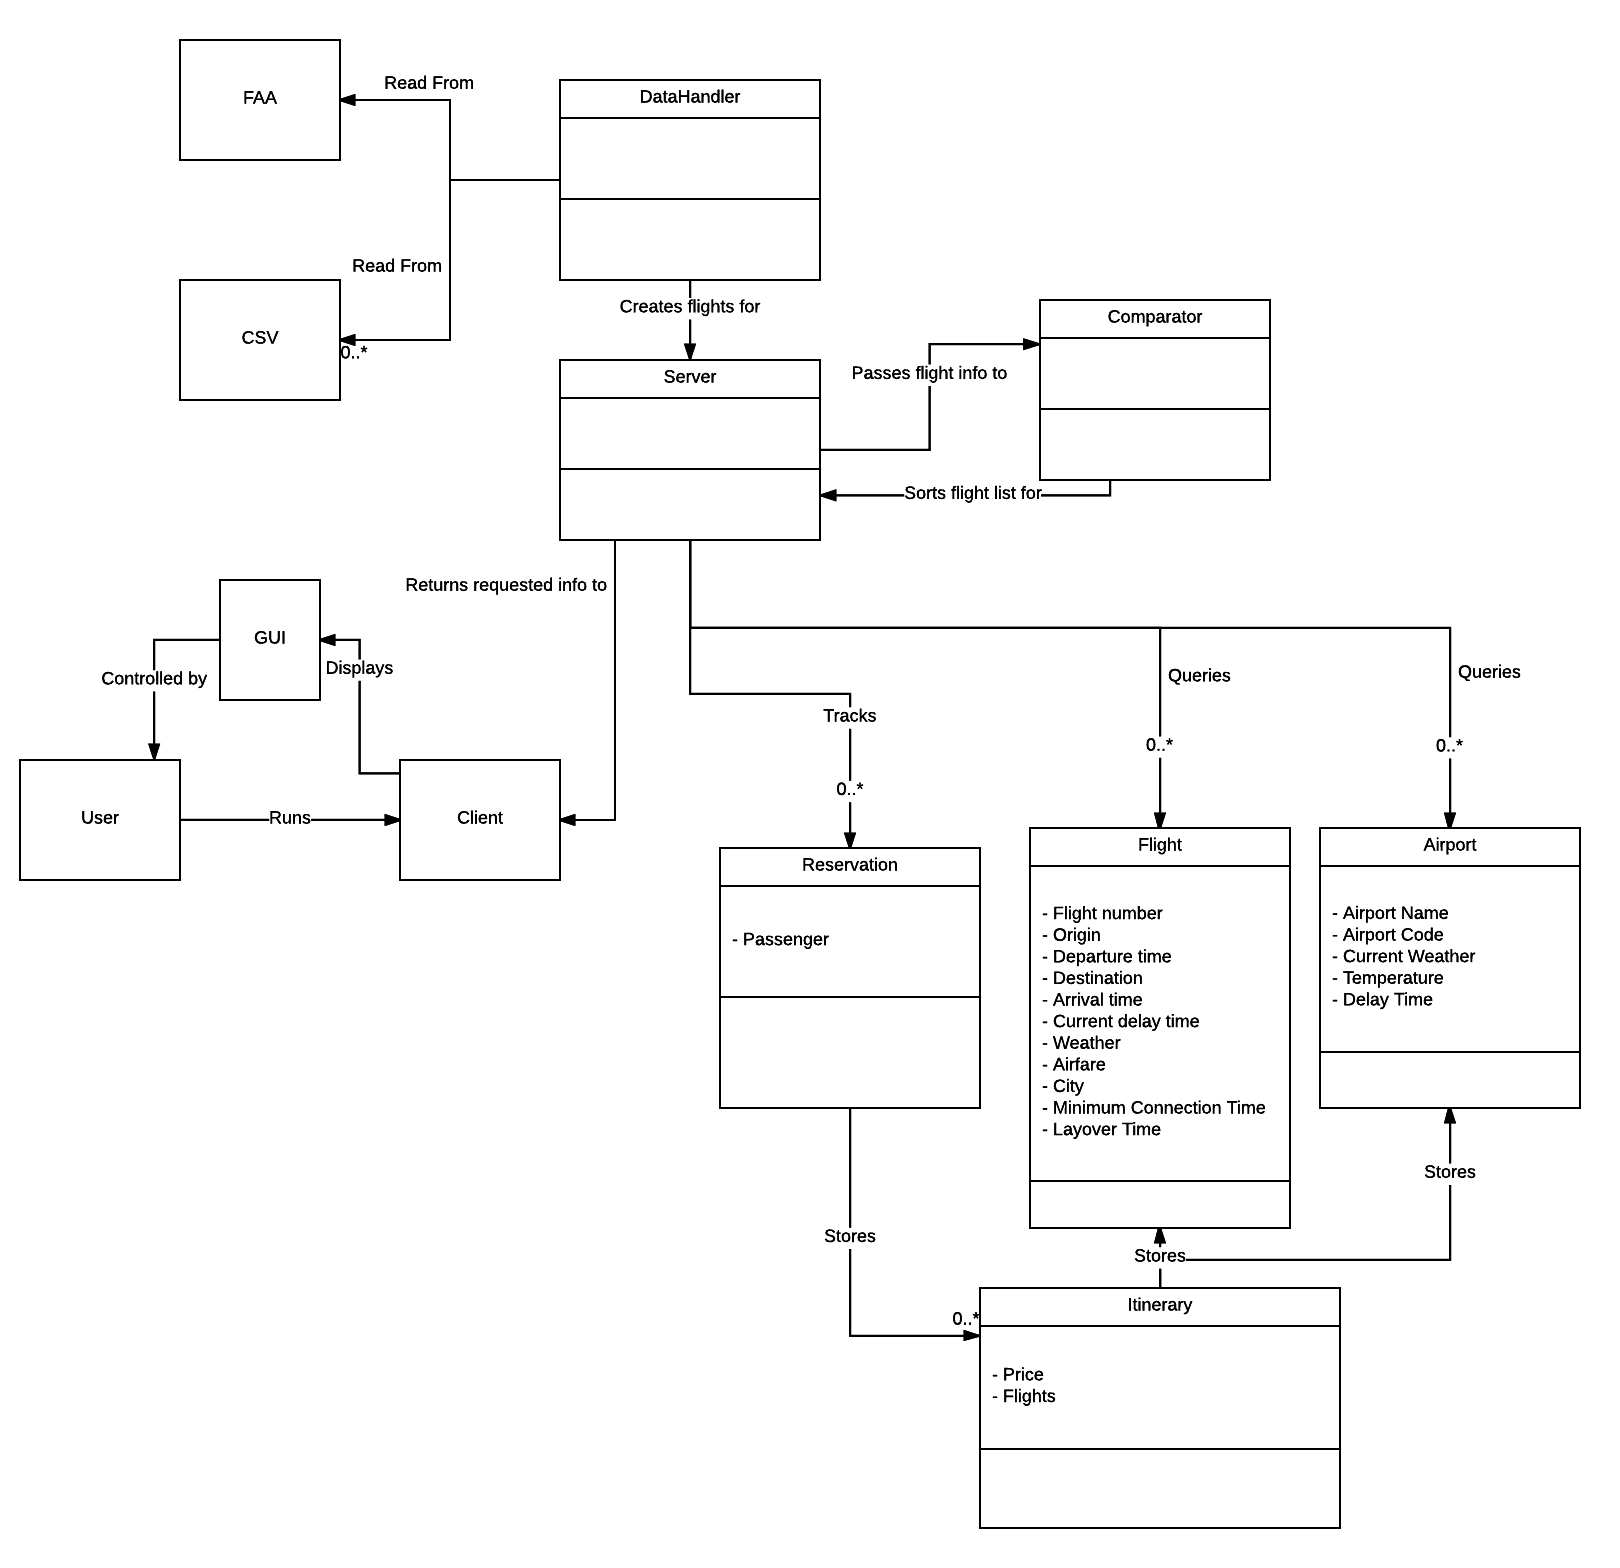
\includegraphics[width=\linewidth]{images/r2domainmodel.png}}
    \end{center}

    %-------------------------------------------------------------------------------
    % System Architecture
    %-------------------------------------------------------------------------------
    \newpage
    \section*{System Architecture}\label{sec:systemArchitecture}
    \addcontentsline{toc}{section}{System Architecture}

    \paragraph{Release 1}

    \indent
    At the end of Release 1, we had a large, complex system that was heavily coupled to the AFRS and Datahandler classes.
    This was made abundantly clear by the fact that when the refactor to the new design was made, the AFRS class was importing a little over half of the classes that had been built in the system.

    \begin{center}
        \makebox[\textwidth]{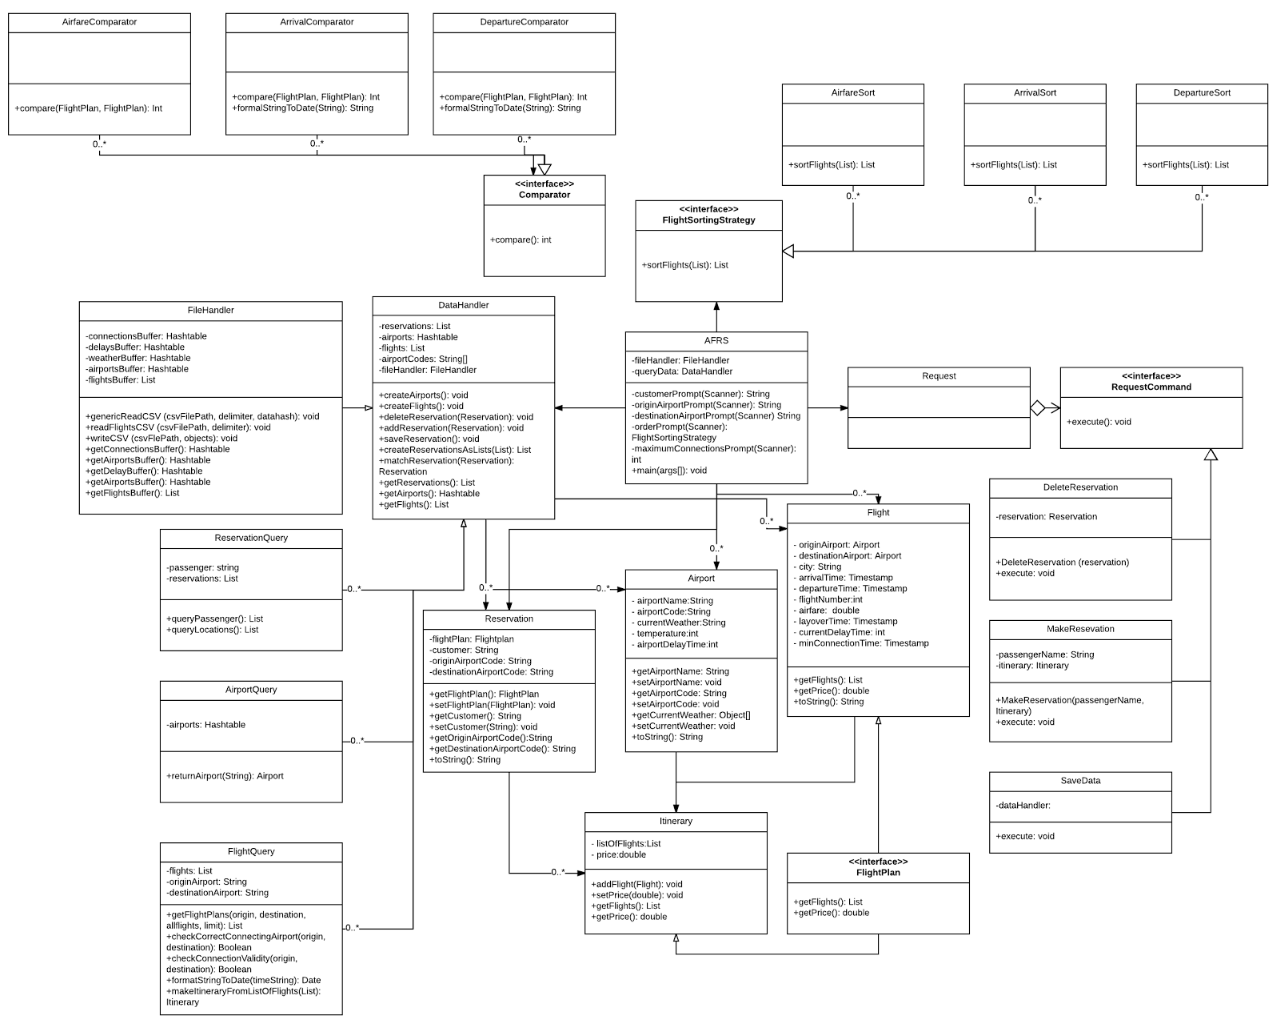
\includegraphics[width=\linewidth]{images/r1class.png}}
    \end{center}

    \newpage

    \paragraph{Release 2}

    \indent
    As part of the refactor the design was coupled away from the AFRS class and began the split into the 3 client/server/common systems.
    This design choice was made in order to decouple the system and allow for multiple concurrent clients with ease.
    There can be as many clients as needed, as long as the server is running as well.
    The Server is the most complex of the three major subsystems.
    A nice benefit of creating this subsystem is decoupling Data Handler and File Handler from some classes that required it in release 1.

    \begin{center}
        \makebox[\textwidth]{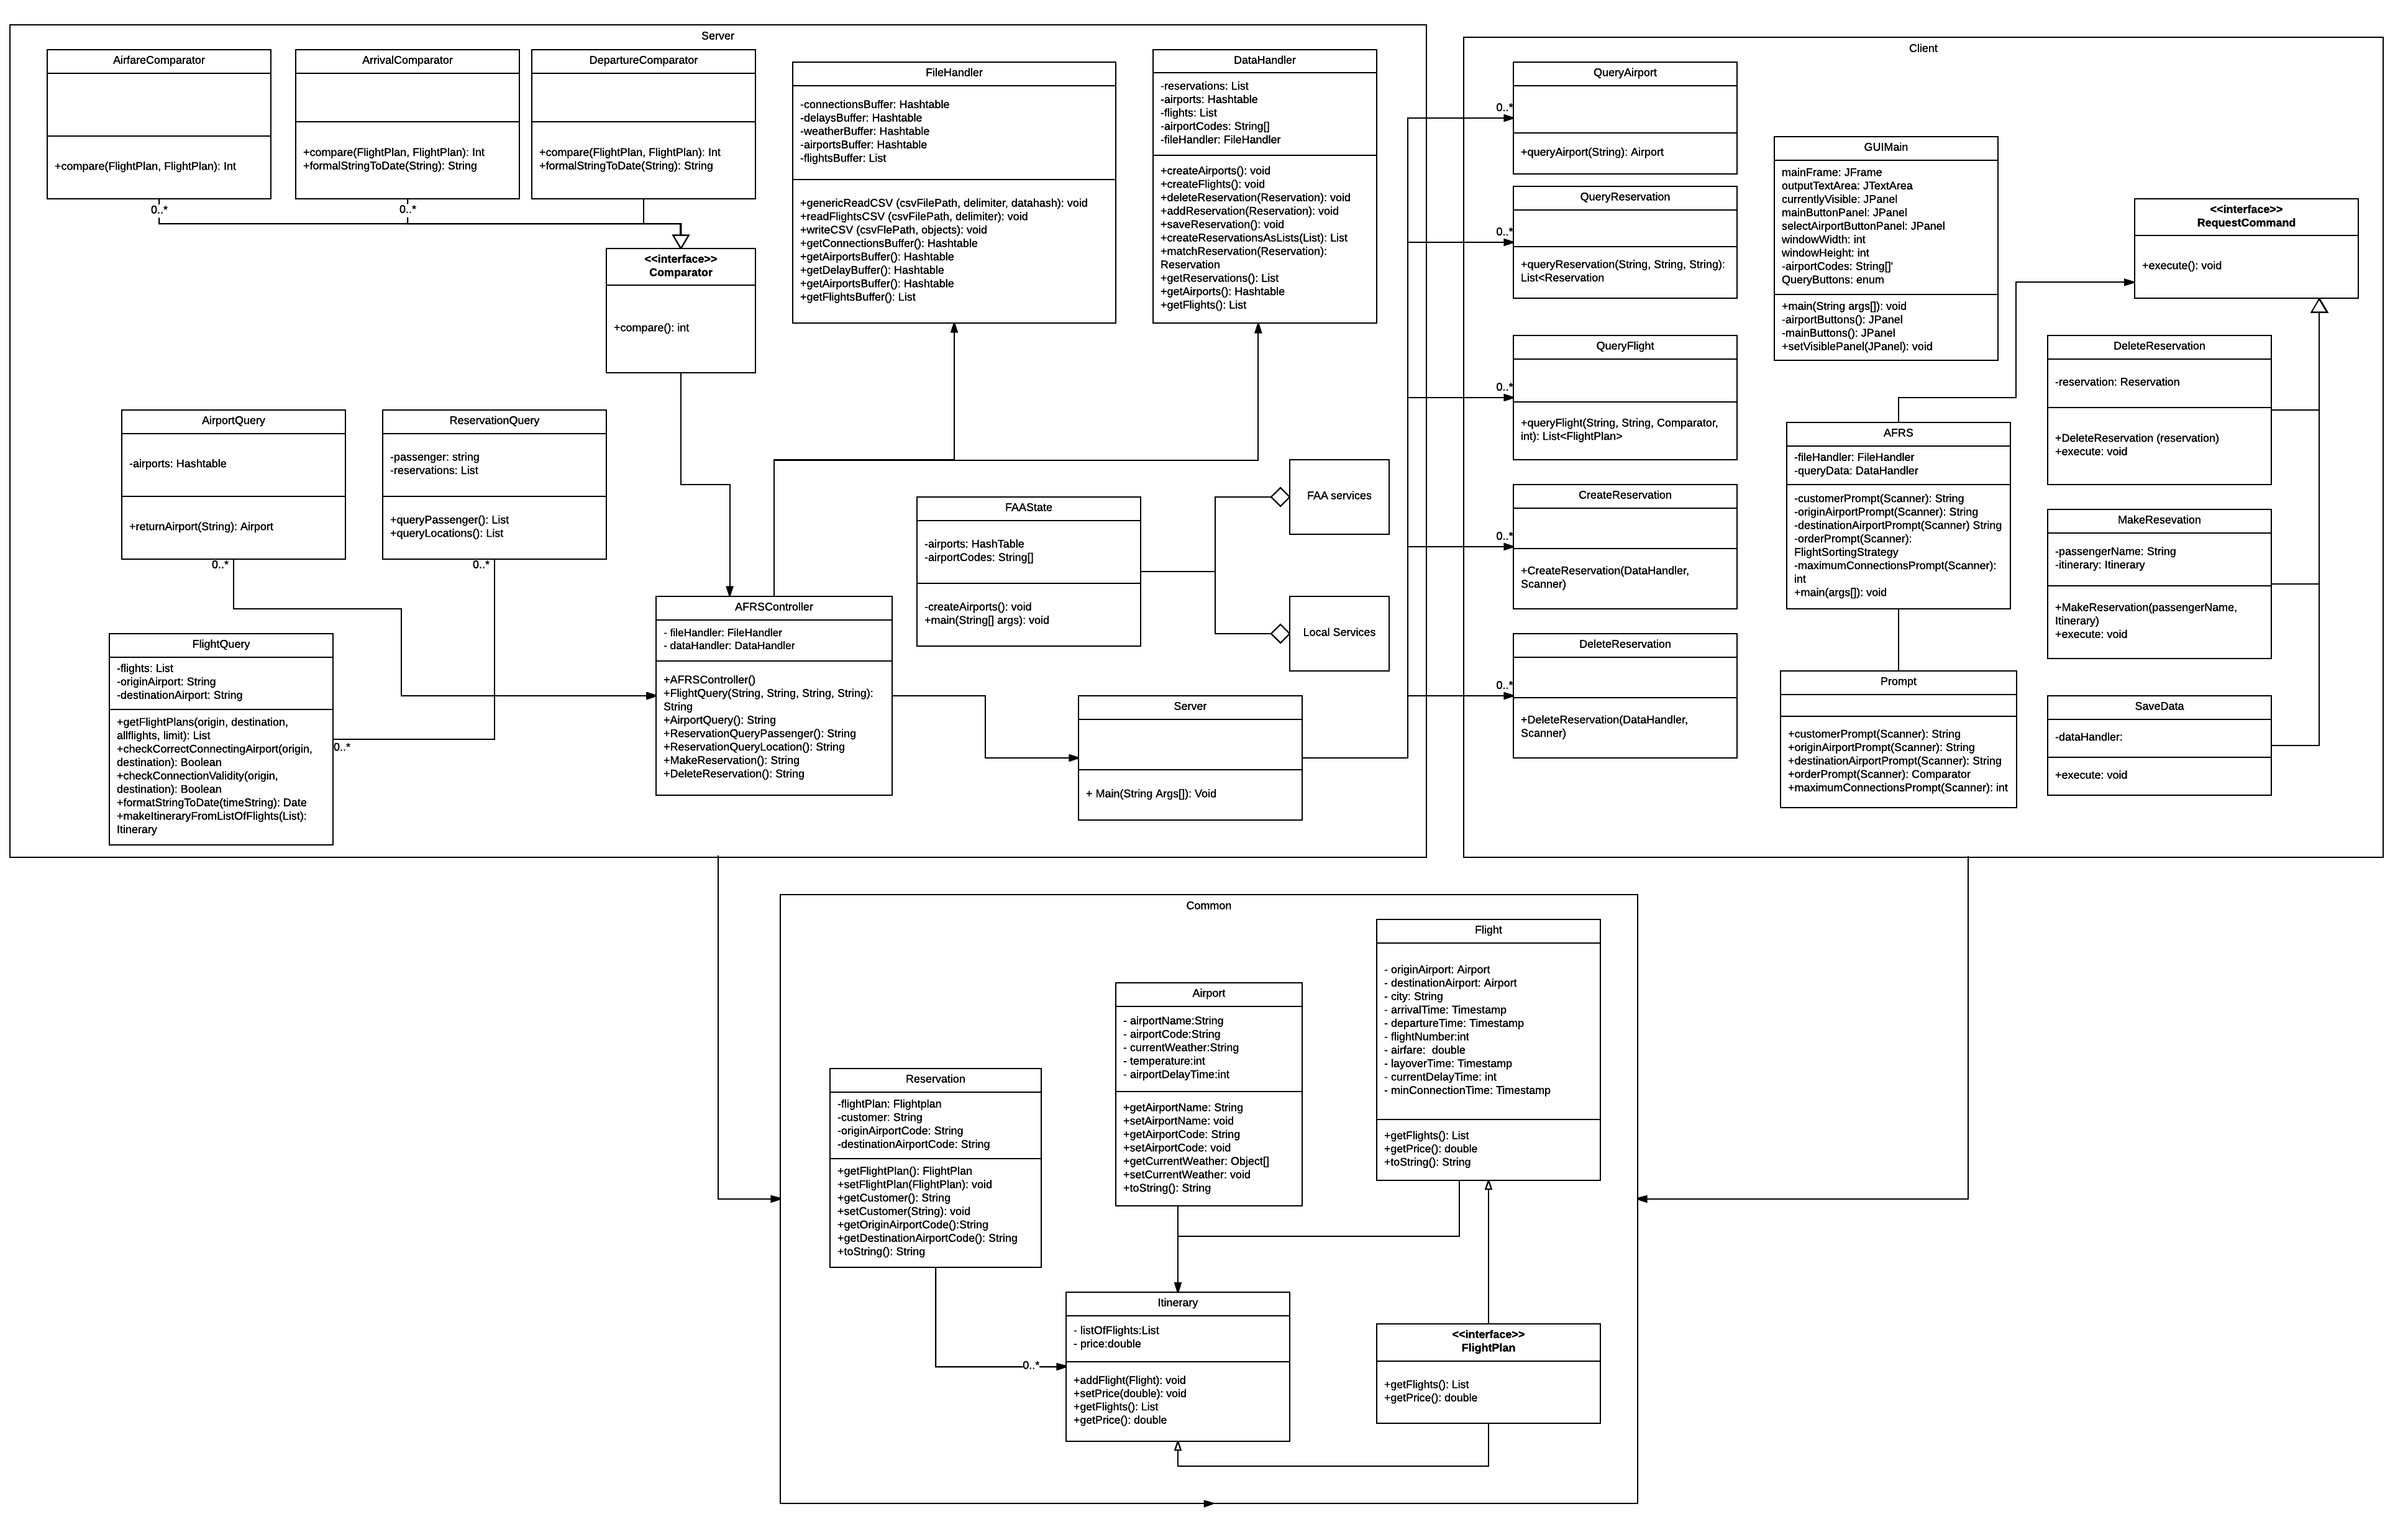
\includegraphics[width=\linewidth]{images/r2classdiagram.png}}
    \end{center}


    %-------------------------------------------------------------------------------
    % Subsystems
    %-------------------------------------------------------------------------------
    \newpage
    \section*{Subsystems}\label{sec:subsystems}
    \addcontentsline{toc}{section}{Subsystems}

%-------------------------------------------------------------------------------
% Subsystems / Client Requests
%-------------------------------------------------------------------------------
\subsection{Client Requests}\label{subsec:clientRequests}

\subsubsection{Class Diagram}
\paragraph{Release 1}

\indent
In release 1, the client had 3 actions that could make through the request classes.
They could make, delete or save reservations.
The requirements only required that the user was able to make and delete a reservation, and that it would persist throughout the system.
In order to make up for the fact that undo was not present in the system, saving the reservations was a separate command to allow for not saving changes that were not wanted.
This was also a pretty poor implementation of the command pattern, as the invoker was never used, and each command was instantiated and removed at use.

\begin{center}
    \makebox[\textwidth]{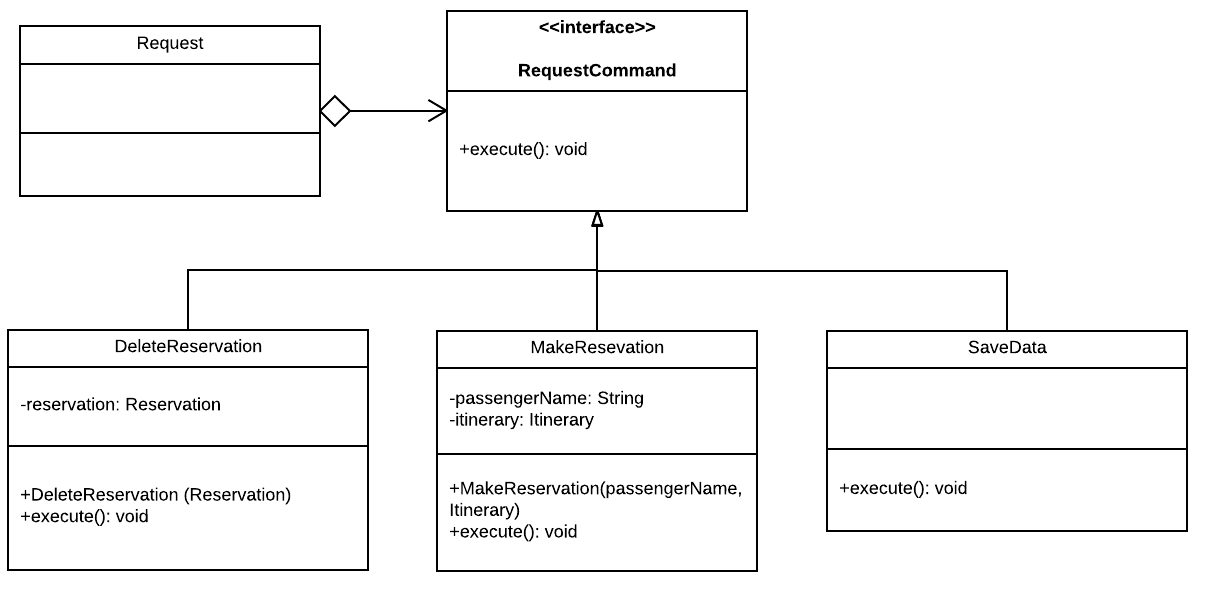
\includegraphics[width=\linewidth]{images/r1request.png}}
\end{center}

\paragraph{Release 2}

\indent
During release 2, the command pattern is moved around and used in a few places.
The requests from Release 1, are still in the client, and provide the undo/redo functionality as they are now meant to by the requirements.
However now they no longer interact with the datahandler directly, they now call routes in the server to perform commands.
Completely invisible to the user, or the client, the actions are then performed on the server.
Now as well as providing a command pattern, this section of the design also provides a proxy pattern for giving the client a place to hit, before all actions are done elsewhere.
A design choice made was to use the command and proxy patterns heavily modified here in order to make it work as we designed.

\subsubsection{Sequence Diagrams}

\paragraph{Release 1}

\begin{center}
    \makebox[\textwidth]{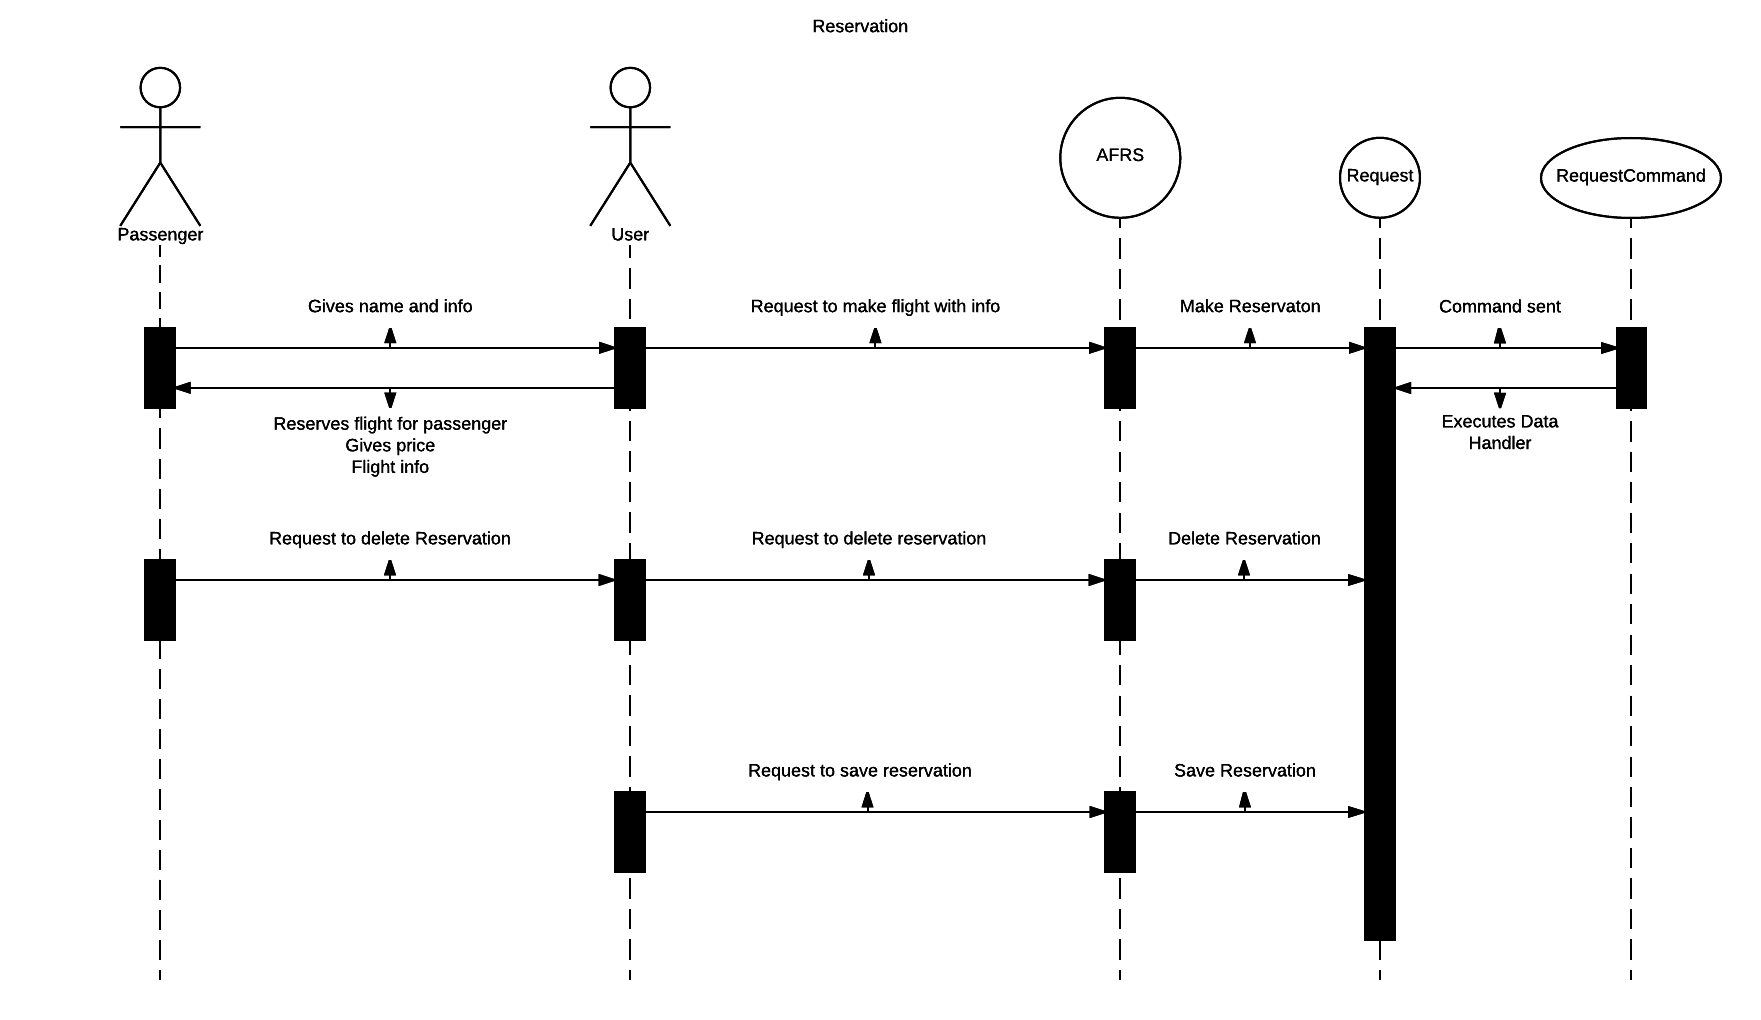
\includegraphics[width=\linewidth]{images/r1sequence1.png}}
\end{center}

\paragraph{Release 2}

\indent
In Release 2 we omitted the Invoker entirely as it was unnecessary. We also had to now account for undoing of commands. With this in mind, it was actually pretty easy to implement simple undo/redo functionality as long as we held a request object in memory to allow us to call the undo/execute commands.

\begin{center}
    \makebox[\textwidth]{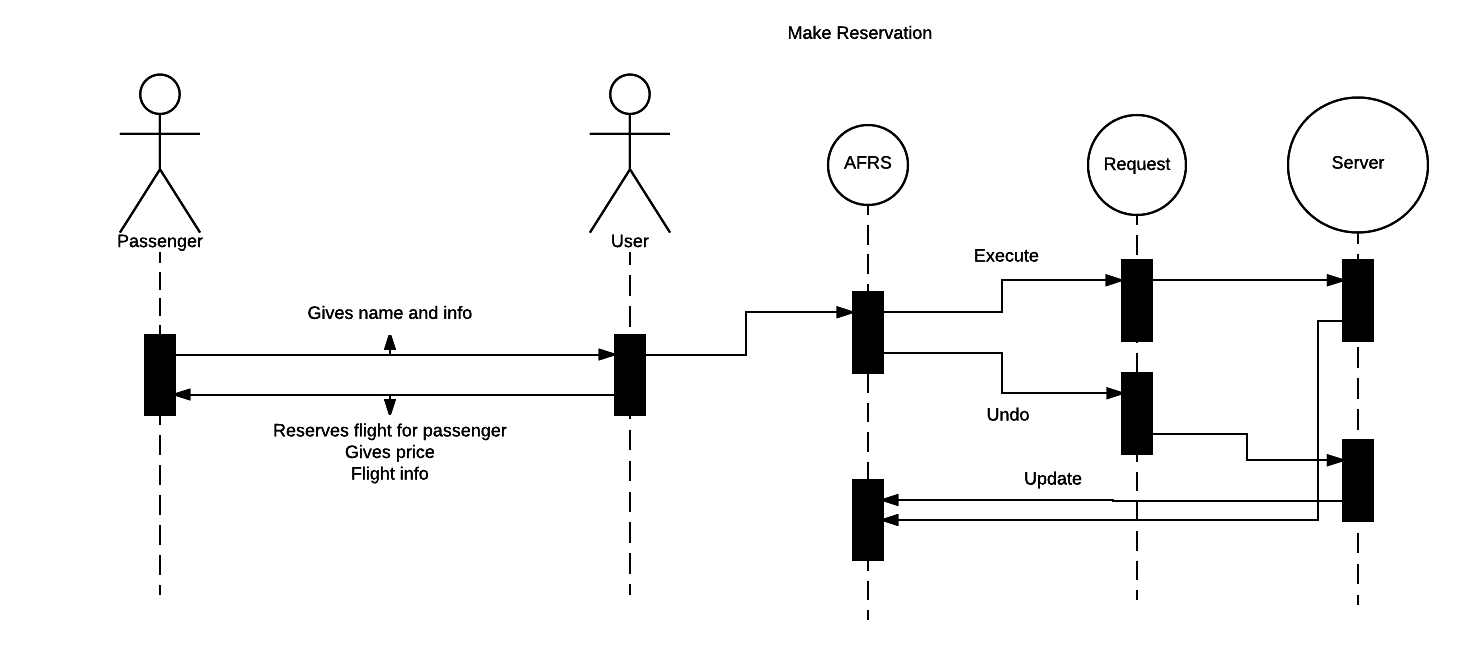
\includegraphics[width=\linewidth]{images/r2-makereservation-sequence.png}}
\end{center}

\subsubsection{GoF Card}
\begin{center}
    \begin{tabular}{ |p{4cm}|p{4cm}|p{7cm}|  }
        \hline
        \multicolumn{2}{|c|}{Name: Request} & \multicolumn{1}{|c|}{GoF pattern: Command} \\
        \hline
        \multicolumn{3}{|c|}{Participants} \\
        \hline
        Class & Role in GoF pattern & Participant's contribution in the context of the application \\
        \hline \hline
        RequestCommand & Command & The overall command which could be used to reuse an existing request as another one.
        Although not currently used in this fashion, it would be fairly easy to make the change. \\
        \hline
        MakeReservation & Concrete Command & Makes a new reservation object and adds it to the system.
        This does so without returning anything to the user, or informing the user about what commands are being performed. \\
        \hline
        DeleteReservation & Concrete Command & Deletes reservation object from the system.
        This does so by calling the class in the datahandler without exposing that to the invoker. \\
        \hline
        \hline
        \multicolumn{3}{|c|}{Deviations from the Pattern:} \\ \multicolumn{3}{|c|}{\parbox{0.9\textwidth}{
        \begin{itemize}
            \item No reflection/pointers involved for target method.
            \item Commands have more distinct methods.
            \item No Invoker class.
        \end{itemize} }} \\
        \hline
        \multicolumn{3}{|c|}{Requirements being covered:} \\ \multicolumn{3}{|c|}{\parbox{0.9\textwidth}{
        \begin{itemize}
            \item The AFRS shall track reservations.
            \item The system shall allow a client to make a reservation for an itinerary contained in the most recent query for flight information.
            \item The system shall allow a client to query for reservations for a passenger.
            \item The system shall allow a client to delete a reservation for a passenger.
        \end{itemize} }} \\
        \hline
    \end{tabular}
\end{center}

\newpage

%-------------------------------------------------------------------------------
% Subsystems / Itineraries
%-------------------------------------------------------------------------------
\subsection{Itineraries}\label{subsec:itineraries}

\subsubsection{Class Diagram}

\paragraph{Release 1 \& 2}

\indent
The design for Flights and Itineraries is one of the subsystems that is the most easily understood.
Flights and Itineraries share a common interface, and therefore can be used interchangeably by the rest of the system.
This use of the composite pattern is incredibly useful here, and because of that, no changes were made between R1 and R2.

\begin{center}
    \makebox[\textwidth]{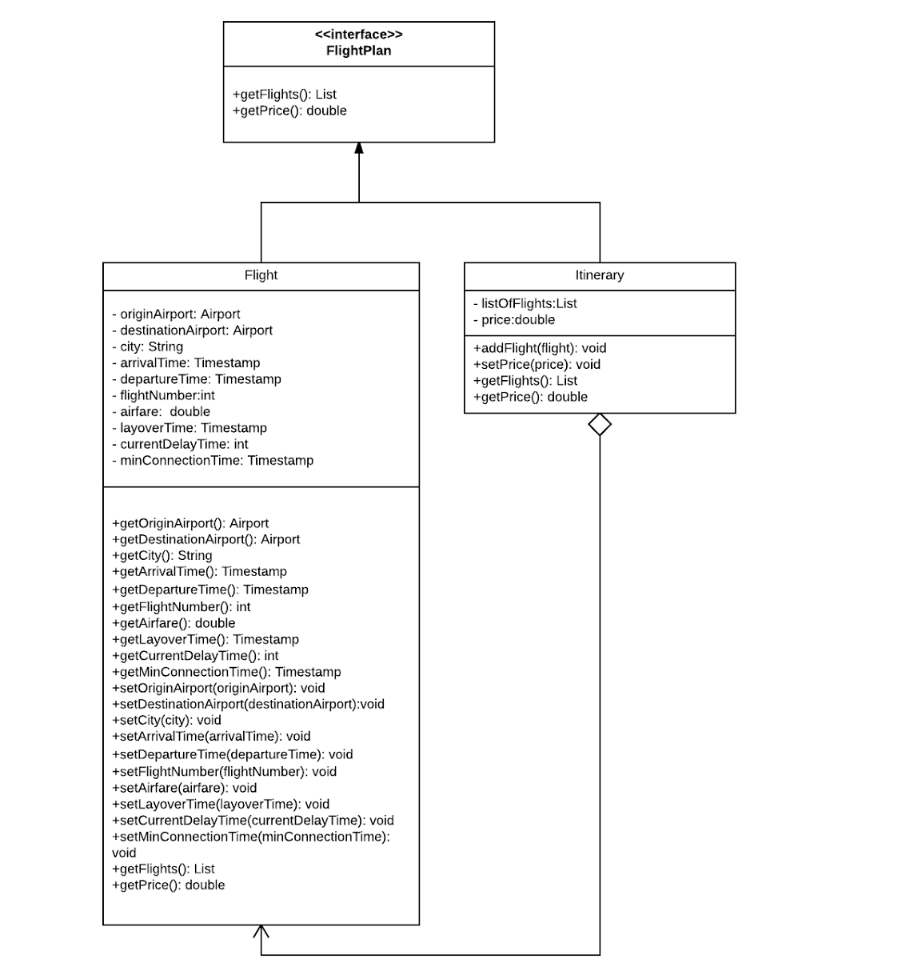
\includegraphics[width=\linewidth]{images/r1itineraries.png}}
\end{center}

\subsubsection{Sequence Diagrams}

\paragraph{Release 1 \& 2}

\indent
In Release 2, we added server route functionality to this subsystem in order to fit it in with the multi-concurrent user system.

\begin{center}
    \makebox[\textwidth]{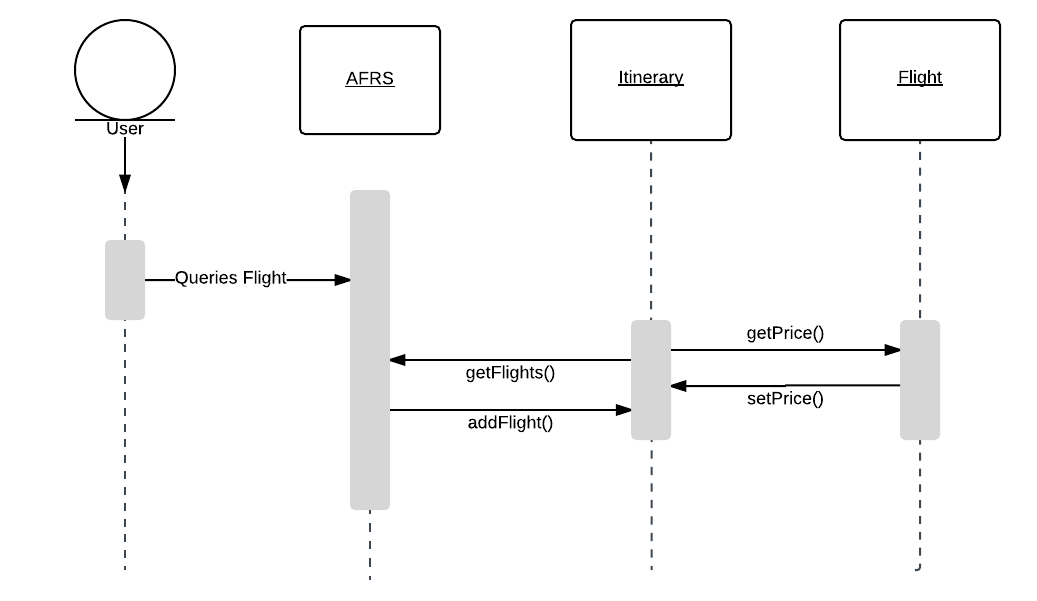
\includegraphics[width=\linewidth]{images/r1itinerarysequence.png}}
\end{center}

\newpage
\subsubsection{GoF Card}

\begin{center}
    \begin{tabular}{ |p{4cm}|p{4cm}|p{7cm}|  }
        \hline
        \multicolumn{2}{|c|}{Name: Itineraries} & \multicolumn{1}{|c|}{GoF pattern: Composite} \\
        \hline
        \multicolumn{3}{|c|}{Participants} \\
        \hline
        Class & Role in GoF pattern & Participant's contribution in the context of the application \\
        \hline \hline
        Flight Plan & Component & The component interface to uniform the leaf and composite. \\
        \hline
        Flight & Leaf & The actual flight object as it exists in the database.
        This will include all information needed to understand a flight. \\
        \hline
        Itinerary & Composite & The itinerary object, with a list of flights, and the total price for each of the flights inside of it.
        This itinerary is a possible set of flights to get from one destination to another. \\
        \hline
        \hline
        \multicolumn{3}{|c|}{Deviations from the Pattern:} \\ \multicolumn{3}{|c|}{\parbox{0.9\textwidth}{
        \begin{itemize}
            \item Leaf has many more encapsulated attributes than composite element.
            \item Composite does not contain Composites. It will only contain leafs.
        \end{itemize} }} \\
        \hline
        \multicolumn{3}{|c|}{Requirements being covered:} \\ \multicolumn{3}{|c|}{\parbox{0.9\textwidth}{
        \begin{itemize}
            \item The system shall store flight data for all flights between the cities in TTA's route network.
            Flight data shall consist of: origin airport, destination airport, departure time, arrival time, flight number, and airfare.
            An itinerary is a list of Flights that also stores the total airfare of each flight.
            This is used when a client creates a reservation with multiple legs.
        \end{itemize} }} \\
        \hline
    \end{tabular}
\end{center}

\newpage

%-------------------------------------------------------------------------------
% Subsystems / Sorting Algorithms
%-------------------------------------------------------------------------------
\subsection{Sorting Algorithms}

\subsubsection{Class Diagram}

\paragraph{Release 1 \& 2}

\indent
In Release 1, there were a series of classes whose sole purpose was to return a comparator.
During the discussion over the R1 design, it was determined that those extra classes were unnecessary to the use of the strategy pattern.
This was creating a series of classes that served no extra functionality, and simply abstracted a part of the system that never needed to be abstracted.

\begin{center}
    \makebox[\textwidth]{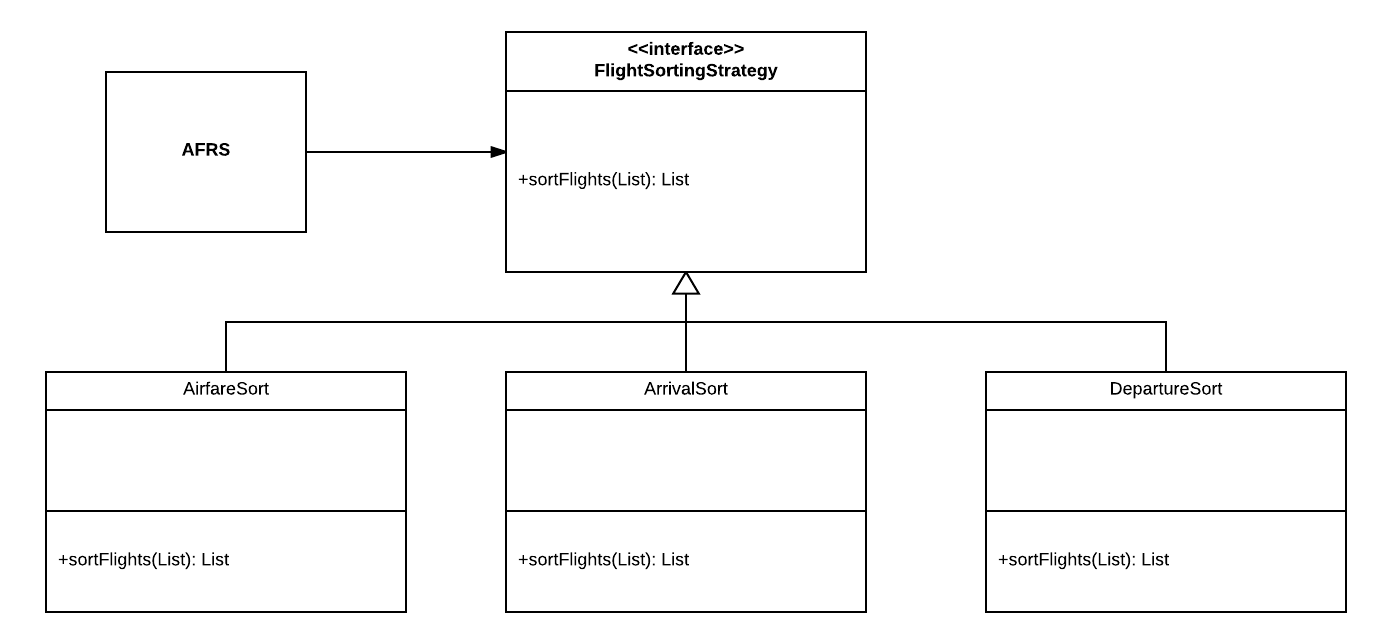
\includegraphics[width=\linewidth]{images/r1sortingclass.png}}
\end{center}

\newpage

\subsubsection{Sequence Diagrams}

\paragraph{Release 1 \& 2}

\begin{center}
    \makebox[\textwidth]{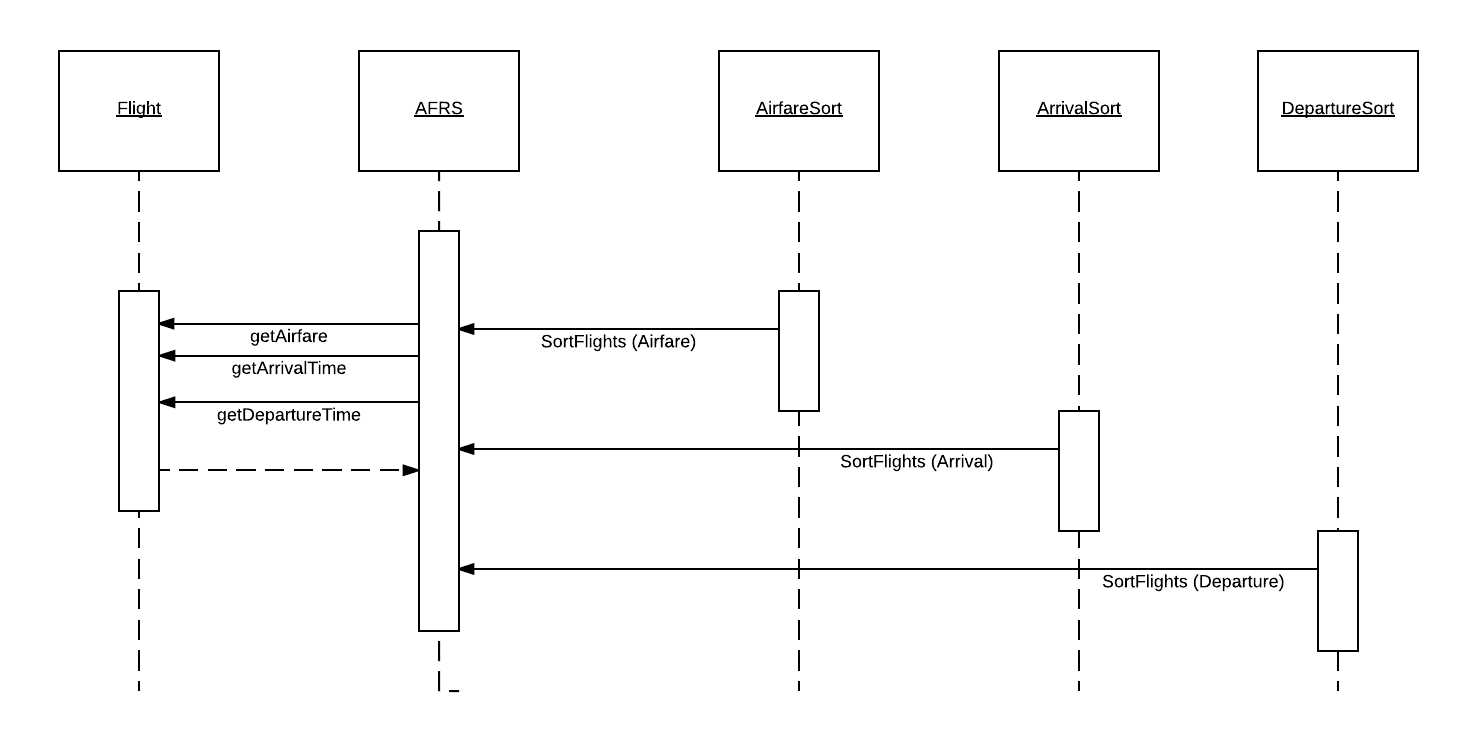
\includegraphics[width=\linewidth]{images/r1sortingstate.png}}
\end{center}

\newpage

\subsubsection{GoF Card}

\begin{center}
    \begin{tabular}{ |p{4cm}|p{4cm}|p{7cm}|  }
        \hline
        \multicolumn{2}{|c|}{Name: Sorting Algorithms} & \multicolumn{1}{|c|}{GoF pattern: Strategy} \\
        \hline
        \multicolumn{3}{|c|}{Participants} \\
        \hline
        Class & Role in GoF pattern & Participant's contribution in the context of the application \\
        \hline \hline

        AFRS & Context & Executes the strategy \\
        \hline
        FlightSortingStrategy & Strategy & An interface for multiple strategies for sorting flights \\
        \hline
        AirfareSort & ConcreteStrategyA & An algorithm for sorting airfare.
        It orders all flights and itineraries by using a Comparator implementation that compares price of two flights.
        Flights are ordered from least to most expensive. \\
        \hline
        ArrivalSort & ConcreteStrategyB & An algorithm for sorting arriving times.
        It orders FlightPlans by using a Comparator implementation that compares the Date objects of the last flight in the FlightPlan’s arrival time.  \\
        \hline
        DepartureSort & ConcreteStrategyC & An algorithm for sorting departing times.
        Using an implementation of the Comparator interface that compares two Date objects for the departure of the first flight in a FlightPlan.  \\
        \hline

        \hline
        \multicolumn{3}{|c|}{Deviations from the Pattern:} \\ \multicolumn{3}{|c|}{\parbox{0.9\textwidth}{
        \begin{itemize}
            \item Each algorithm essentially does the same work with a different comparator rather than a completely different algorithm.
            However, the client still has the power to change a backend algorithm and it is done on the fly.
        \end{itemize} }} \\
        \hline
        \multicolumn{3}{|c|}{Requirements being covered:} \\ \multicolumn{3}{|c|}{\parbox{0.9\textwidth}{
        \begin{itemize}
            \item Sorting of Flights and Itineraries given an option to sort them.
        \end{itemize} }} \\
        \hline
    \end{tabular}
\end{center}

\newpage

%-------------------------------------------------------------------------------
% Subsystems / Proxy
%-------------------------------------------------------------------------------
\subsection{Proxy}\label{subsec:proxy}

\indent
In the transition to a client-server subsystem, we implemented a controller for the user to request information.
With the proxy pattern, the system gives the client methods they can call, then translates that call to server.
This way, the client doesn’t need to know where the data is or how to explicitly fetch it.

\subsubsection{Class Diagram}

\paragraph{Release 2}

\begin{center}
    \makebox[\textwidth]{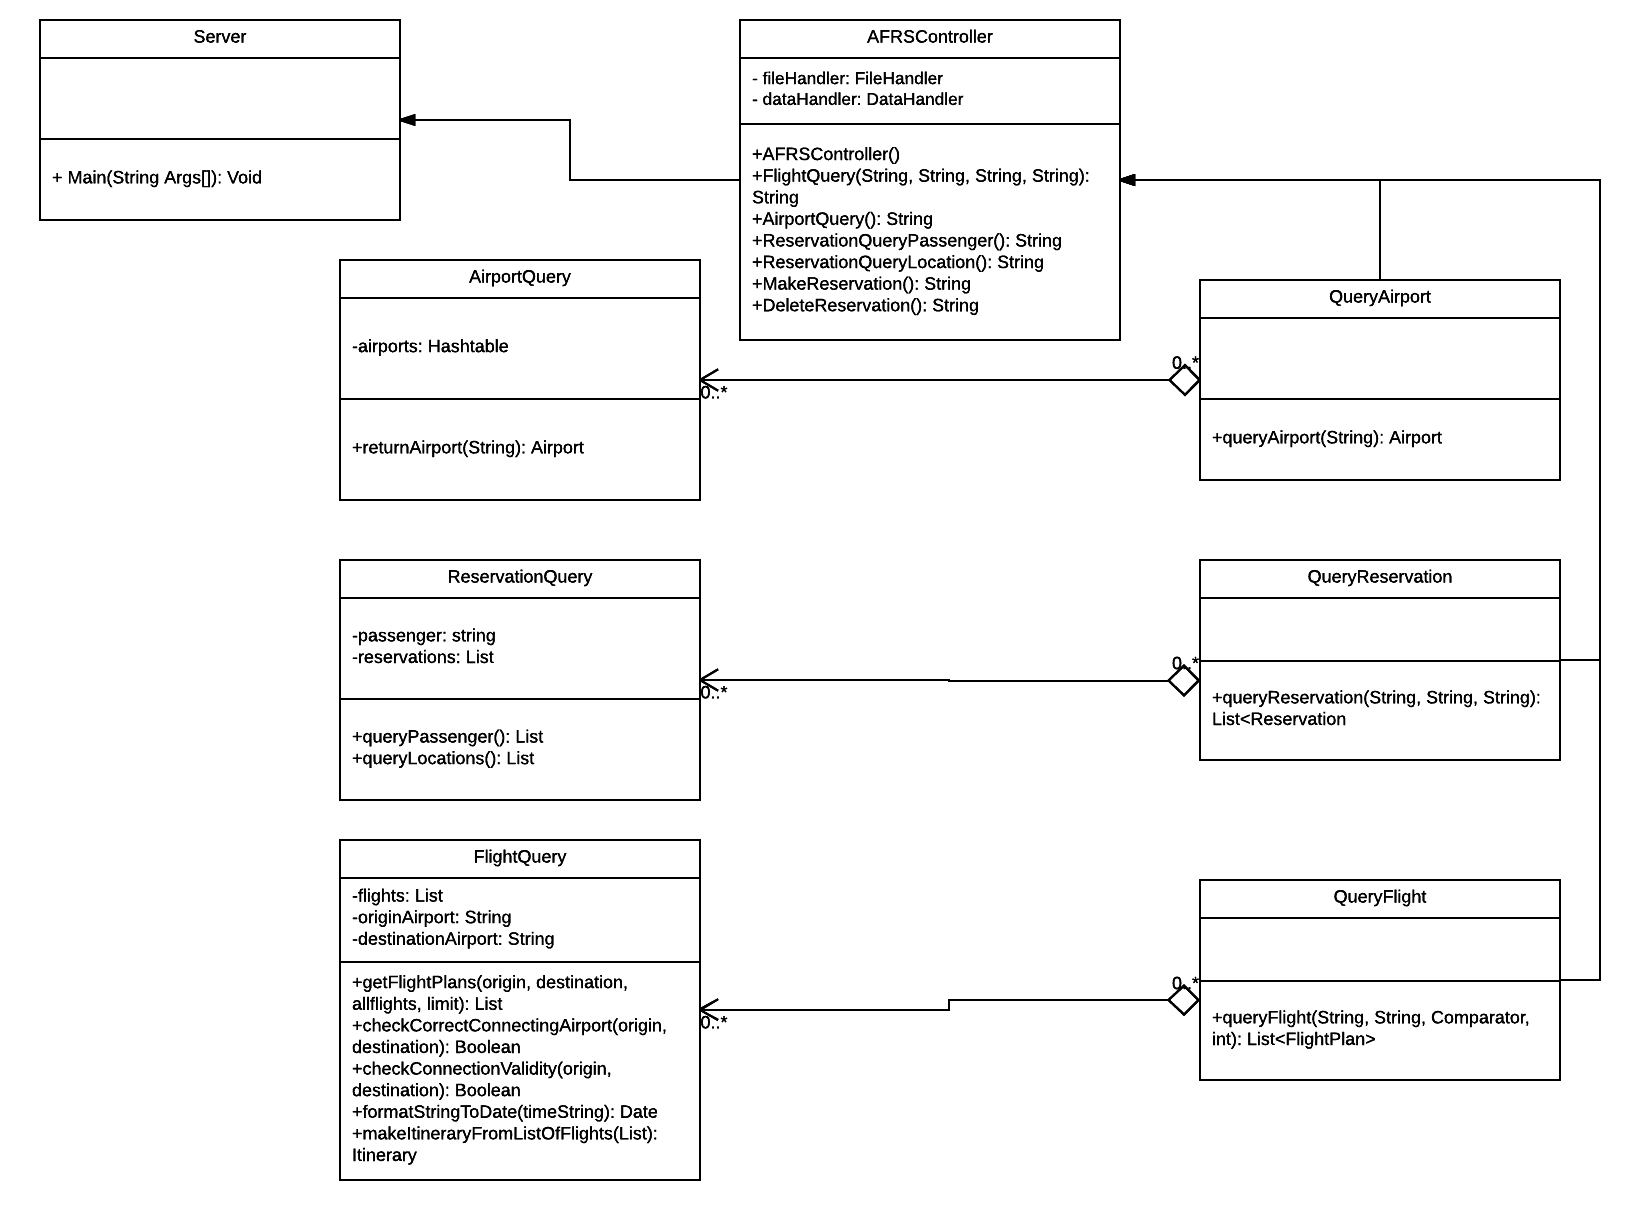
\includegraphics[width=\linewidth]{images/r2-proxy-class.png}}
\end{center}

\newpage

\subsubsection{Sequence Diagrams}

\paragraph{Release 2}

\begin{center}
    \makebox[\textwidth]{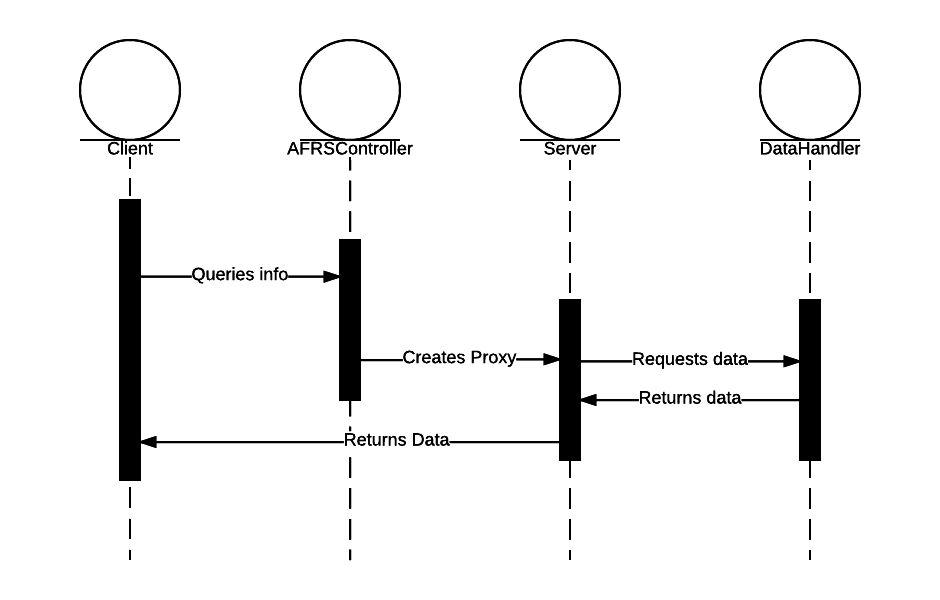
\includegraphics[width=\linewidth]{images/r2-proxy-sequence.png}}
\end{center}

\newpage

\subsubsection{GoF Card}

\begin{center}
    \begin{tabular}{ |p{4cm}|p{4cm}|p{7cm}|  }
        \hline
        \multicolumn{2}{|c|}{Name: Proxy} & \multicolumn{1}{|c|}{GoF pattern: Proxy} \\
        \hline
        \multicolumn{3}{|c|}{Participants} \\
        \hline
        Class & Role in GoF pattern & Participant's contribution in the context of the application \\
        \hline \hline

        CreateReservationProxy & Proxy & Makes a call to the Make Reservation Route on the server to create a reservation with the matching object information.\\
        \hline
        /MakeReservationQuery & Real Subject & Route for performing the actual reservation creation. This is done on the server regardless of which client made the request. Once it has made the request, all clients will be able to see this reservation in the system.\\
        \hline
        DeleteReservationProxy & Proxy & Makes a call to the Delete Reservation Route on the server to delete the reservation matching the object information sent over.\\
        \hline
        /DeleteReservationQuery & Real Subject & Route for performing the actual reservation deletion. This is done on the server regardless of which client made the request. Once it has deleted the reservation all clients will no longer be able to see the reservation in the system.\\
        \hline
        QueryAirport & Proxy &
        Makes a call to the Airport Query on the Server and returns the airport object that the server returns
        \\
        \hline
    \end{tabular}
    \begin{tabular}{ |p{4cm}|p{4cm}|p{7cm}|  }
        \hline
        Class & Role in GoF pattern & Participant's contribution in the context of the application \\
        \hline \hline
        /AirportQuery & Real Subject &
        Searches either the FAA or local files to return the airport object of the request, then returns it.
        \\
        \hline
        QueryFlight & Proxy &
        Makes a call to the Flight Query on the server and receives the flights and itineraries that exist on the server given the information provided.
        \\
        \hline
        /FlightQuery & Real Subject &
        Searches through its collection of flights and itineraries to return a list of FlightPlans to the client making the request.
        \\
        \hline
        QueryReservation & Proxy &
        Makes a call to the Query Reservation on the server and recieves Reservations given a passenger name.
        \\
        \hline
        /ReservationQueryPassenger & Real Subject &
        Searches through existing reservations for any reservations matching the queried passenger name and returns all matching objects to the client.
        \\
        \hline

        \hline
        \multicolumn{3}{|c|}{Deviations from the Pattern:} \\ \multicolumn{3}{|c|}{\parbox{0.9\textwidth}{
        \begin{itemize}
            \item Proxy and subject classes do not implement an interface.
        \end{itemize} }} \\
        \hline
        \multicolumn{3}{|c|}{Requirements being covered:} \\ \multicolumn{3}{|c|}{\parbox{0.9\textwidth}{
        \begin{itemize}
            \item The AFRS supports multiple clients but not truly concurrent clients.
        \end{itemize} }} \\
        \hline
    \end{tabular}
\end{center}

\newpage

%-------------------------------------------------------------------------------
% Subsystems / RESTFul Web Service
%-------------------------------------------------------------------------------
\subsection{RESTFul Web Service}\label{subsec:restfulWebService2}

One significant issue coming from release 1 was the coupling of our queries to the data handler.
With the introduction of a new multi-user requirement, we implemented a Facade Pattern, having our server controller (AFRSController) serve as the facade for all server subsystems to interact in one place.
What keeps it from being anti-pattern is how it is coupled;
none of the subsystems need to know about AFRSController, while direct coupling between queries and datahandler is kept minimal.

\subsubsection{Class Diagram}

\paragraph{Release 2}

\begin{center}
    \makebox[\textwidth]{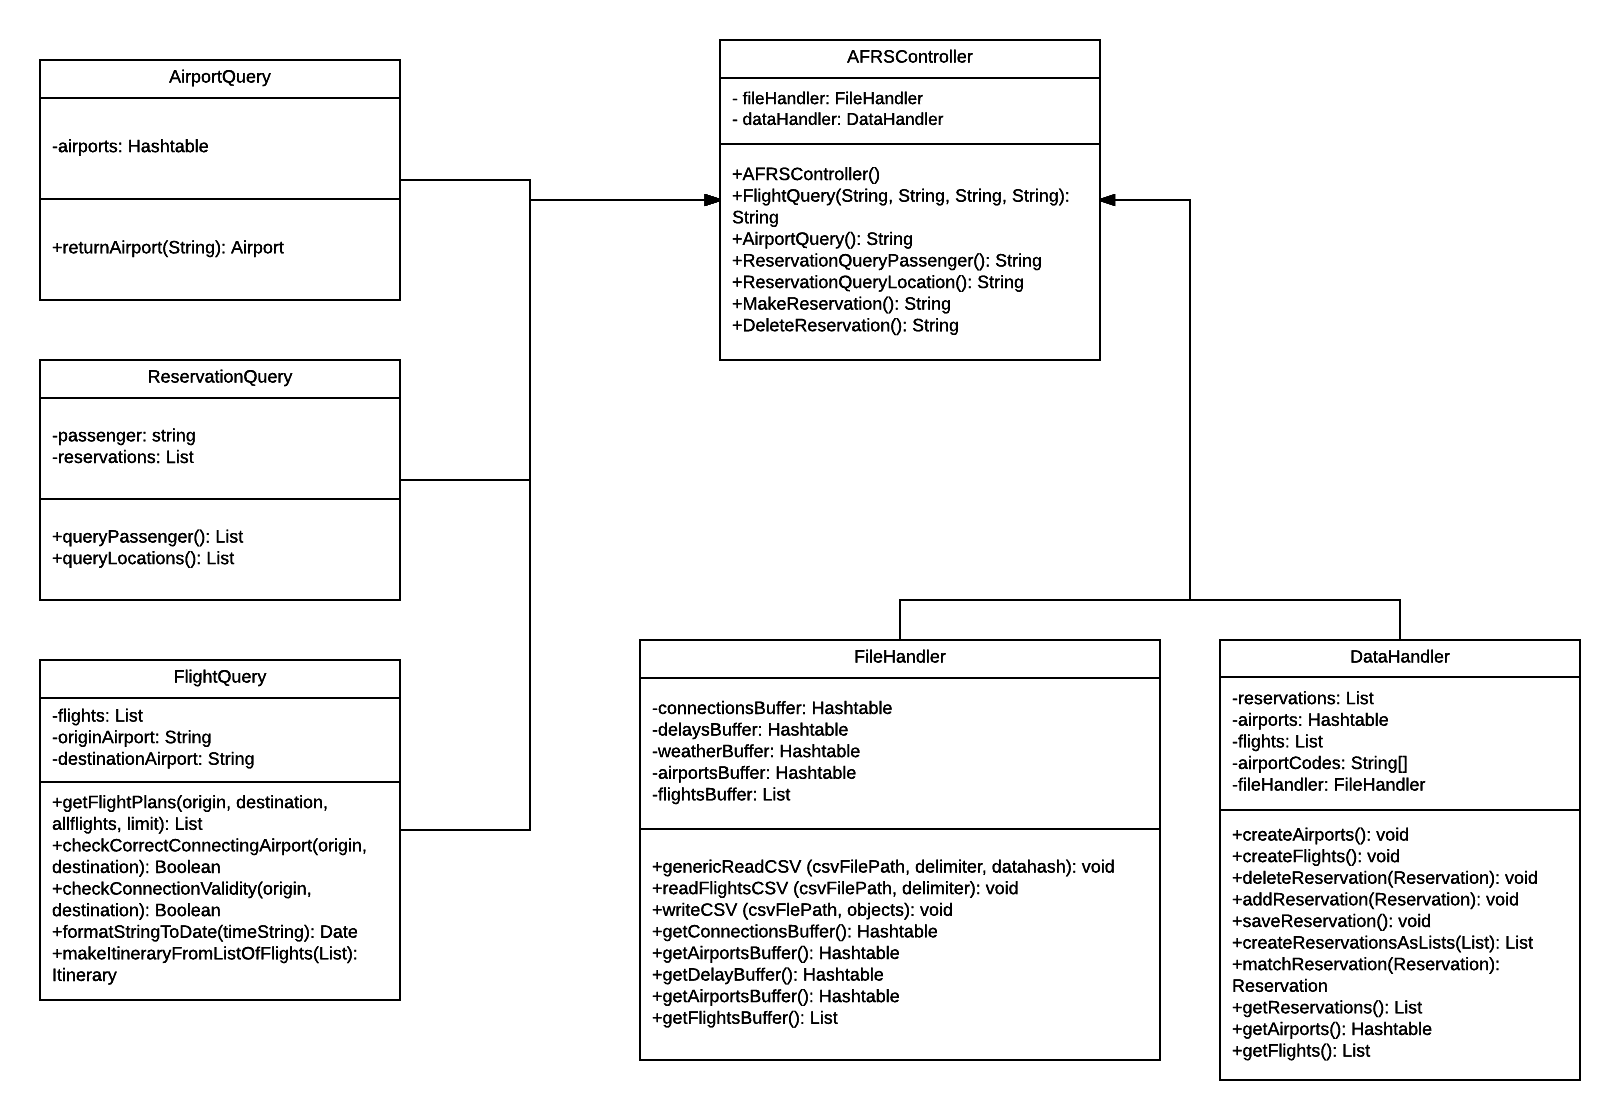
\includegraphics[width=\linewidth]{images/r2-AFRScontroller-class.png}}
\end{center}

\newpage

\subsubsection{Sequence Diagrams}

\paragraph{Release 2}

\begin{center}
    \makebox[\textwidth]{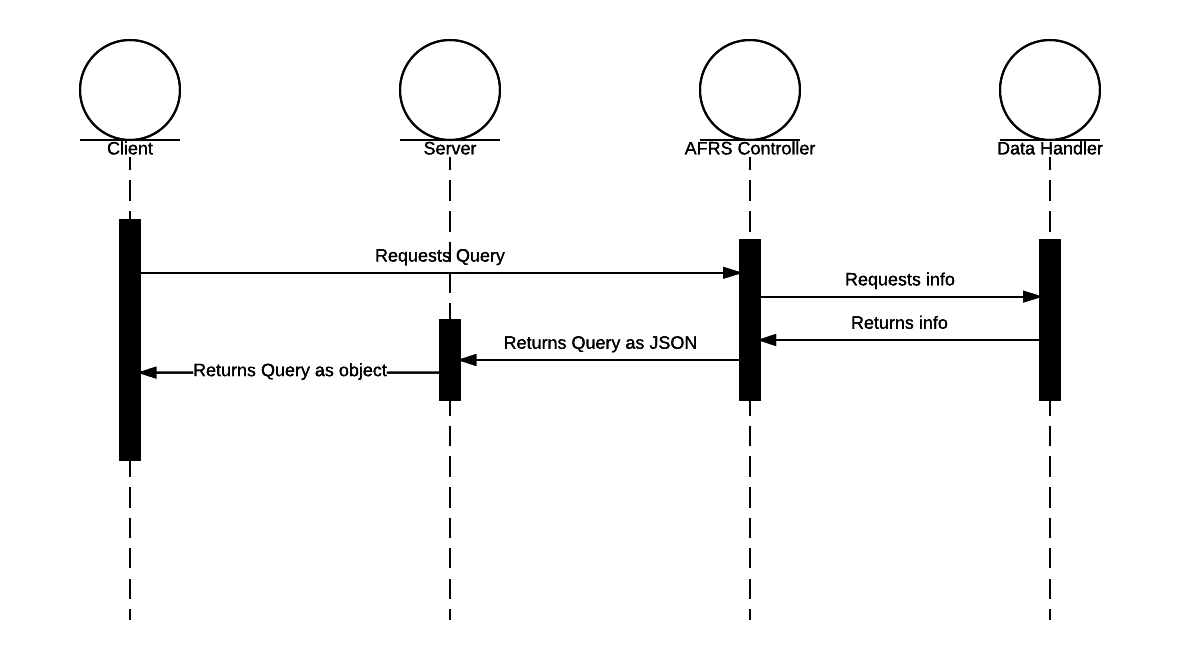
\includegraphics[width=\linewidth]{images/r2-AFRScontroller-sequence.png}}
\end{center}

\newpage

\subsubsection{GoF Card}

\begin{center}
    \begin{tabular}{ |p{4cm}|p{4cm}|p{7cm}|  }
        \hline
        \multicolumn{2}{|c|}{Name: RESTFul Web Service} & \multicolumn{1}{|c|}{GoF pattern: Facade} \\
        \hline
        \multicolumn{3}{|c|}{Participants} \\
        \hline
        Class & Role in GoF pattern & Participant's contribution in the context of the application \\
        \hline \hline

        AFRSController & Facade & Encapsulates all queries with datahandler and calls queries server-side using the datahandler. \\
        \hline
        AirportQuery & SubsystemA &
        Returns an airport object
        \\
        \hline
        ReservationQuery & SubsystemA &
        Returns a list of reservations by passenger name or origin and destination airports
        \\
        \hline
        FlightQuery & SubsystemA &
        Returns a list of flight plans
        \\
        \hline
        DataHandler & SubsystemB &
        Provides queried data from local or FAA
        \\
        \hline

        \hline
        \multicolumn{3}{|c|}{Deviations from the Pattern:} \\ \multicolumn{3}{|c|}{\parbox{0.9\textwidth}{
        \begin{itemize}
            \item SubsystemB’s DataHandler is instantiated in the SubsystemA classes directly for construction.
            \item Facade does add some new functionality related to server interaction
            \item Facade is not an interface
        \end{itemize} }} \\
        \hline
        \multicolumn{3}{|c|}{Requirements being covered:} \\ \multicolumn{3}{|c|}{\parbox{0.9\textwidth}{
        \begin{itemize}
            \item Server and client interactions enabling multi-concurrent users.
        \end{itemize} }} \\
        \hline
    \end{tabular}
\end{center}

\newpage

%-------------------------------------------------------------------------------
% Subsystems / FAA or Local State
%-------------------------------------------------------------------------------
\subsection{FAA or Local State}\label{subsec:faaOrLocalState}

\indent
One new requirement in R2 was to allow the user to fetch information from FAA services instead of local. The system initially loads from local anyway, which we believed made it a good fit for the State Pattern. It has an obvious default state (local) and can transition to FAA on request and back. Additionally it only loads local by default, which makes the system load faster than having to load both simultaneously (in case the user never wishes to fetch from FAA). This also makes state transitions after the first one faster since local and FAA remain loaded.

\subsubsection{Class Diagram}

\paragraph{Release 2}

\begin{center}
    \makebox[\textwidth]{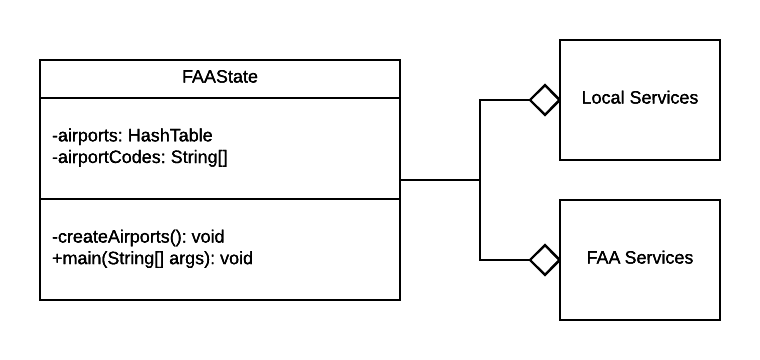
\includegraphics[width=\linewidth]{images/R2-FAA-State.png}}
\end{center}

\subsubsection{State Diagram}

\paragraph{Release 2}

\begin{center}
    \makebox[\textwidth]{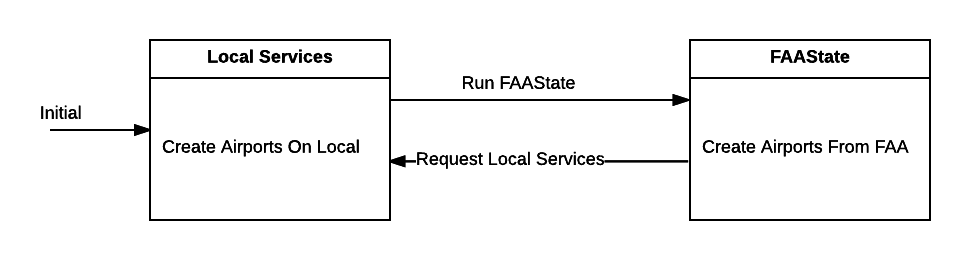
\includegraphics[width=\linewidth]{images/r2-FAA-state.png}}
\end{center}

\subsubsection{Sequence Diagrams}

\paragraph{Release 2}

\begin{center}
    \makebox[\textwidth]{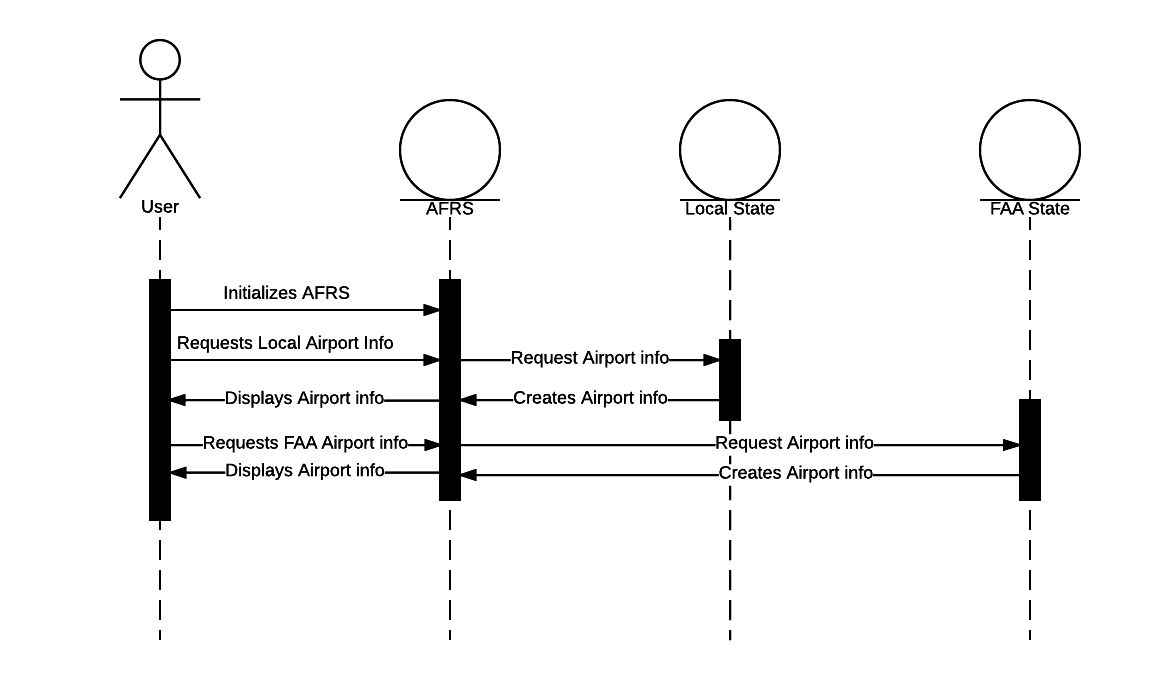
\includegraphics[width=\linewidth]{images/r2-FAA-sequence.png}}
\end{center}

\subsubsection{GoF Card}

\begin{center}
    \begin{tabular}{ |p{4cm}|p{4cm}|p{7cm}|  }
        \hline
        \multicolumn{2}{|c|}{Name: FAA or Local State} & \multicolumn{1}{|c|}{GoF pattern: State} \\
        \hline
        \multicolumn{3}{|c|}{Participants} \\
        \hline
        Class & Role in GoF pattern & Participant's contribution in the context of the application \\
        \hline \hline

        FAAState & ConcreteState &
        Enables system to read data from FAA service only if the client requests it.
        \\
        \hline

        \hline
        \multicolumn{3}{|c|}{Deviations from the Pattern:} \\ \multicolumn{3}{|c|}{\parbox{0.9\textwidth}{
        \begin{itemize}
            \item State does not implement an interface
        \end{itemize} }} \\
        \hline
        \multicolumn{3}{|c|}{Requirements being covered:} \\ \multicolumn{3}{|c|}{\parbox{0.9\textwidth}{
        \begin{itemize}
            \item Provides the user the ability to view airport information either from local services or FAA.
        \end{itemize} }} \\
        \hline
    \end{tabular}
\end{center}

\newpage
    

    %-------------------------------------------------------------------------------
    % Status of the Implementation
    %-------------------------------------------------------------------------------
    \section*{Status of the Implementation}\label{sec:statusOfTheImplementation}
    \addcontentsline{toc}{section}{Status of the Implementation}

    \indent
    Overall the implementation is about minimizing places for user error.
    Out system decided against doing single string requests and instead went for a series of prompts to the user to create a request that cannot be made incomplete.
    Partial requests are eliminated.
    There is no need for semicolons (;).
    With these things in mind most of the logic can exist on the backend instead of up front on the user interface.


    \subsection*{User Interface Implementation}\label{subsec:userInterfaceImplementation}
    \begin{itemize}
        \item Text interface provides users a sequence of preset options. The reasons we implemented it this way are:
        \begin{itemize}
            \item This eliminates the need for the user to memorize commands.
            \item Request process is sped up.
            \item This reduces the possibility for input error (spelling, format, accidental termination).
            \item Less testing is needed.
        \end{itemize}
        \item GUI interface is available to alleviate the fallbacks of using a terminal based interface.
        \begin{itemize}
            \item User input is handled by more mouse clicks than keyboard input
            \item Errors are reduced by prompts being provided with clearer displays
        \end{itemize}
    \end{itemize}

    \subsection*{CSV Implementation}\label{subsec:csvImplementation}
    \begin{itemize}
        \item A small subsystem was created to handle data read/writes.
        This system stores data in hash tables as an alternative to database:
        \begin{itemize}
            \item A FileHandler class reads from CSVs and writes to other CSVs.
            \item A DataHandler class holds methods to manipulate data from FileHandler (i.e Flights, Reservations)
        \end{itemize}
    \end{itemize}

    \subsection*{Client/Server/Common}\label{subsec:client/server/common}
    \begin{itemize}
        \item After the release of Release 1, the system was split into client, server and common systems.
        This design change meaning that no classes inside client were used by server, and vice versa, with the only classes being shared being from common.
        \begin{itemize}
            \item This decouples client and server.
        \end{itemize}
    \end{itemize}

    \subsection*{RESTful Web Service}\label{subsec:restfulWebService}
    \begin{itemize}
        \item Our choice for handling multiple concurrent user support was implementing Spring RESTful Web Service via Gradle.
        \begin{itemize}
            \item This simplified creating routes heavily.
            Every command has a small route implementation to return a parsable JSON representation.
            \item We decided this outweighed the difficulty of integrating Gradle into our project.
        \end{itemize}
    \end{itemize}

    %-------------------------------------------------------------------------------
    % Appendix
    %-------------------------------------------------------------------------------
    \newpage
    \section*{Appendix}\label{sec:appendix}
    \addcontentsline{toc}{section}{Appendix}

%-------------------------------------------------------------------------------
% Common
%-------------------------------------------------------------------------------
\subsection{Common}\label{subsec:common}

\begin{center}
    \begin{tabular}{ |p{7cm}|p{7cm}|  }
        \hline
        \multicolumn{2}{|c|}{Class: Airport} \\
        \hline
        \multicolumn{2}{|c|}{Responsibilities:} \\ \multicolumn{2}{|c|}{\parbox{0.9\textwidth}{
        \begin{itemize}
            \item Object to store all information about each Airport.
        \end{itemize} }} \\
        \hline
        \multicolumn{2}{|c|}{Collaborators:} \\
        \hline
        Users: & Used by: AirportQuery, DataHandler, AFRS, AFRSController \\
        \hline
        \multicolumn{2}{|c|}{Author: Devin Matte} \\
        \hline
        \multicolumn{2}{|c|}{Package: Models} \\
        \hline
    \end{tabular}
\end{center}


\begin{center}
    \begin{tabular}{ |p{7cm}|p{7cm}|  }
        \hline
        \multicolumn{2}{|c|}{Class: Flight} \\
        \hline
        \multicolumn{2}{|c|}{Responsibilities:} \\ \multicolumn{2}{|c|}{\parbox{0.9\textwidth}{
        \begin{itemize}
            \item Object to store all information about any given flight to use in building itineraries and reservations
        \end{itemize} }} \\
        \hline
        \multicolumn{2}{|c|}{Collaborators:} \\
        \hline
        Users: FlightPlan & Used by: Itinerary, AFRSController \\
        \hline
        \multicolumn{2}{|c|}{Author: Amanda Ramos} \\
        \hline
        \multicolumn{2}{|c|}{Package: Models} \\
        \hline
    \end{tabular}
\end{center}


\begin{center}
    \begin{tabular}{ |p{7cm}|p{7cm}|  }
        \hline
        \multicolumn{2}{|c|}{Class: Itinerary} \\
        \hline
        \multicolumn{2}{|c|}{Responsibilities:} \\ \multicolumn{2}{|c|}{\parbox{0.9\textwidth}{
        \begin{itemize}
            \item Collect a series of flights to make a full flight including connections from one airport to another.
        \end{itemize} }} \\
        \hline
        \multicolumn{2}{|c|}{Collaborators:} \\
        \hline
        Users: Flight, FlightPlan & Used by: DataHandler, FlightQuery, AFRSController \\
        \hline
        \multicolumn{2}{|c|}{Author: Nicholas Montemorano, Devin Matte} \\
        \hline
        \multicolumn{2}{|c|}{Package: Models} \\
        \hline
    \end{tabular}
\end{center}


\begin{center}
    \begin{tabular}{ |p{7cm}|p{7cm}|  }
        \hline
        \multicolumn{2}{|c|}{Class: Reservation} \\
        \hline
        \multicolumn{2}{|c|}{Responsibilities:} \\ \multicolumn{2}{|c|}{\parbox{0.9\textwidth}{
        \begin{itemize}
            \item A flight, or itinerary of flights for a customer to fly. Has the customer, origin, destination and corresponding flight plan
        \end{itemize} }} \\
        \hline
        \multicolumn{2}{|c|}{Collaborators:} \\
        \hline
        Users: Flight, FlightPlan & Used by: AFRS, DataHandler, AFRSController \\
        \hline
        \multicolumn{2}{|c|}{Author: Nicholas Montemorano, Oren Rosin} \\
        \hline
        \multicolumn{2}{|c|}{Package: Models} \\
        \hline
    \end{tabular}
\end{center}

%-------------------------------------------------------------------------------
% Server
%-------------------------------------------------------------------------------
\subsection{Server}\label{subsec:server}

\begin{center}
    \begin{tabular}{ |p{7cm}|p{7cm}|  }
        \hline
        \multicolumn{2}{|c|}{Class: AFRSController} \\
        \hline
        \multicolumn{2}{|c|}{Responsibilities:} \\ \multicolumn{2}{|c|}{\parbox{0.9\textwidth}{
        \begin{itemize}
            \item Creates routes for queries made by the client. Queries include Flight plans, Airports, and Reservations as well as executing methods for making and deleting reservations.
        \end{itemize} }} \\
        \hline
        \multicolumn{2}{|c|}{Collaborators:} \\
        \hline
        Users: FlightQuery, AirportQuery, ReservationQuery, DataHandler, FileHandler, Flight, FlightPlan, Itinerary, Resevation, AirfareComparator, ArrivalComparator, DeparatureComparator & Used by: Server \\
        \hline
        \multicolumn{2}{|c|}{Author: Oren Rosin, Devin Matte} \\
        \hline
        \multicolumn{2}{|c|}{Package: RESTfulAPI} \\
        \hline
    \end{tabular}
\end{center}

\begin{center}
    \begin{tabular}{ |p{7cm}|p{7cm}|  }
        \hline
        \multicolumn{2}{|c|}{Class: Server} \\
        \hline
        \multicolumn{2}{|c|}{Responsibilities:} \\ \multicolumn{2}{|c|}{\parbox{0.9\textwidth}{
        \begin{itemize}
            \item Boots Spring Web Service, allowing the routes to be created.
        \end{itemize} }} \\
        \hline
        \multicolumn{2}{|c|}{Collaborators:} \\
        \hline
        Users: AFRSController & Used by: Server \\
        \hline
        \multicolumn{2}{|c|}{Author: Oren Rosin, Devin Matte} \\
        \hline
        \multicolumn{2}{|c|}{Package: RESTfulAPI} \\
        \hline
    \end{tabular}
\end{center}

\begin{center}
    \begin{tabular}{ |p{7cm}|p{7cm}|  }
        \hline
        \multicolumn{2}{|c|}{Class: FileHandler} \\
        \hline
        \multicolumn{2}{|c|}{Responsibilities:} \\ \multicolumn{2}{|c|}{\parbox{0.9\textwidth}{
        \begin{itemize}
            \item Read/Write for CSV files. Stores data in hash tables.
        \end{itemize} }} \\
        \hline
        \multicolumn{2}{|c|}{Collaborators:} \\
        \hline
        Users: None & Used by: AFRSController \\
        \hline
        \multicolumn{2}{|c|}{Author: Nicholas Montemorano} \\
        \hline
        \multicolumn{2}{|c|}{Package: DataHandler} \\
        \hline
    \end{tabular}
\end{center}

\begin{center}
    \begin{tabular}{ |p{7cm}|p{7cm}|  }
        \hline
        \multicolumn{2}{|c|}{Class: DataHandler} \\
        \hline
        \multicolumn{2}{|c|}{Responsibilities:} \\ \multicolumn{2}{|c|}{\parbox{0.9\textwidth}{
        \begin{itemize}
            \item Holds methods to manipulate data in FileHandler
        \end{itemize} }} \\
        \hline
        \multicolumn{2}{|c|}{Collaborators:} \\
        \hline
        Users: Airport, Flight, Itinerary, Reservation & Used by: AFRS, MakeReservation, DeleteReservation \\
        \hline
        \multicolumn{2}{|c|}{Author: Nicholas Montemorano} \\
        \hline
        \multicolumn{2}{|c|}{Package: DataHandler} \\
        \hline
    \end{tabular}
\end{center}

\begin{center}
    \begin{tabular}{ |p{7cm}|p{7cm}|  }
        \hline
        \multicolumn{2}{|c|}{Class: AirfareComparator} \\
        \hline
        \multicolumn{2}{|c|}{Responsibilities:} \\ \multicolumn{2}{|c|}{\parbox{0.9\textwidth}{
        \begin{itemize}
            \item Implements the Comparator interface, meaning it must implement the compare method that returns an integer. It takes two FlightPlan objects, retrieves their airfare and returns a positive or negative integer to indicate which airfare is higher.
        \end{itemize} }} \\
        \hline
        \multicolumn{2}{|c|}{Collaborators:} \\
        \hline
        Users: FlightPlan & Used by: None \\
        \hline
        \multicolumn{2}{|c|}{Author: Nicholas Montemorano} \\
        \hline
        \multicolumn{2}{|c|}{Package: Comparators} \\
        \hline
    \end{tabular}
\end{center}

\begin{center}
    \begin{tabular}{ |p{7cm}|p{7cm}|  }
        \hline
        \multicolumn{2}{|c|}{Class: DepartureComparator} \\
        \hline
        \multicolumn{2}{|c|}{Responsibilities:} \\ \multicolumn{2}{|c|}{\parbox{0.9\textwidth}{
        \begin{itemize}
            \item Implements the Comparator interface by creating a compare method that takes two FlightPlan objects. The FlightPlans contain a departure time as a String. This class converts each date String to a Date object and compares the two, returning a positive or negative integer.
        \end{itemize} }} \\
        \hline
        \multicolumn{2}{|c|}{Collaborators:} \\
        \hline
        Users: FlightPlan & Used by: None \\
        \hline
        \multicolumn{2}{|c|}{Author: Nicholas Montemorano} \\
        \hline
        \multicolumn{2}{|c|}{Package: Comparators} \\
        \hline
    \end{tabular}
\end{center}

\begin{center}
    \begin{tabular}{ |p{7cm}|p{7cm}|  }
        \hline
        \multicolumn{2}{|c|}{Class: ArrivalComparator} \\
        \hline
        \multicolumn{2}{|c|}{Responsibilities:} \\ \multicolumn{2}{|c|}{\parbox{0.9\textwidth}{
        \begin{itemize}
            \item Implements the Comparator interface by creating a compare method that takes two FlightPlan objects. The FlightPlans contain an arrival time of each flight as a String. This class converts the last flight’s date from a string to a Date object and compares the two, returning a positive or negative integer.
        \end{itemize} }} \\
        \hline
        \multicolumn{2}{|c|}{Collaborators:} \\
        \hline
        Users: FlightPlan & Used by: None \\
        \hline
        \multicolumn{2}{|c|}{Author: Nicholas Montemorano} \\
        \hline
        \multicolumn{2}{|c|}{Package: Comparators} \\
        \hline
    \end{tabular}
\end{center}

\begin{center}
    \begin{tabular}{ |p{7cm}|p{7cm}|  }
        \hline
        \multicolumn{2}{|c|}{Class: AirportQueryServer} \\
        \hline
        \multicolumn{2}{|c|}{Responsibilities:} \\ \multicolumn{2}{|c|}{\parbox{0.9\textwidth}{
        \begin{itemize}
            \item Creates and returns an airport object with relevant information to that airport, including name, code, weather, temperature and delay time
        \end{itemize} }} \\
        \hline
        \multicolumn{2}{|c|}{Collaborators:} \\
        \hline
        Users: Datahandler, Airport & Used by: AFRSController \\
        \hline
        \multicolumn{2}{|c|}{Author: Devin Matte} \\
        \hline
        \multicolumn{2}{|c|}{Package: Queries} \\
        \hline
    \end{tabular}
\end{center}

\begin{center}
    \begin{tabular}{ |p{7cm}|p{7cm}|  }
        \hline
        \multicolumn{2}{|c|}{Class: FlightQueryServer} \\
        \hline
        \multicolumn{2}{|c|}{Responsibilities:} \\ \multicolumn{2}{|c|}{\parbox{0.9\textwidth}{
        \begin{itemize}
            \item Creates and returns a list of flight plans, containing information for flight number, origin, destination, and price of each flight.
        \end{itemize} }} \\
        \hline
        \multicolumn{2}{|c|}{Collaborators:} \\
        \hline
        Users: DataHandler, Flight, FlightPlan, Itinerary, DepartureComparator & Used by: AFRSController \\
        \hline
        \multicolumn{2}{|c|}{Author: Devin Matte} \\
        \hline
        \multicolumn{2}{|c|}{Package: Queries} \\
        \hline
    \end{tabular}
\end{center}

\begin{center}
    \begin{tabular}{ |p{7cm}|p{7cm}|  }
        \hline
        \multicolumn{2}{|c|}{Class: ReservationQueryServer} \\
        \hline
        \multicolumn{2}{|c|}{Responsibilities:} \\ \multicolumn{2}{|c|}{\parbox{0.9\textwidth}{
        \begin{itemize}
            \item Creates and returns a list of reservation objects based on either a) the requested passenger name or b) the requested origin and destinations of the reservation.
        \end{itemize} }} \\
        \hline
        \multicolumn{2}{|c|}{Collaborators:} \\
        \hline
        Users: DataHandler, Reservation & Used by: AFRSController \\
        \hline
        \multicolumn{2}{|c|}{Author: Devin Matte} \\
        \hline
        \multicolumn{2}{|c|}{Package: Queries} \\
        \hline
    \end{tabular}
\end{center}

%-------------------------------------------------------------------------------
% Client
%-------------------------------------------------------------------------------
\subsection{Client}\label{subsec:client}

\begin{center}
    \begin{tabular}{ |p{7cm}|p{7cm}|  }
        \hline
        \multicolumn{2}{|c|}{Class: AFRS} \\
        \hline
        \multicolumn{2}{|c|}{Responsibilities:} \\ \multicolumn{2}{|c|}{\parbox{0.9\textwidth}{
        \begin{itemize}
            \item AFRS is the main class. This is what is run when the user runs the program. It prompts for all user input and does most of the input handling.
        \end{itemize} }} \\
        \hline
        \multicolumn{2}{|c|}{Collaborators:} \\
        \hline
        Users: CreateReservationProxy, DeleteReservationProxy QueryAirport, QueryFlight, QueryReservation, Airport, FlightPlan, Reservation, Prompt & Used by: None \\
        \hline
        \multicolumn{2}{|c|}{Author: Devin Matte, Amanda Ramos} \\
        \hline
    \end{tabular}
\end{center}

\begin{center}
    \begin{tabular}{ |p{7cm}|p{7cm}|  }
        \hline
        \multicolumn{2}{|c|}{Class: MakeReservation} \\
        \hline
        \multicolumn{2}{|c|}{Responsibilities:} \\ \multicolumn{2}{|c|}{\parbox{0.9\textwidth}{
        \begin{itemize}
            \item A command which tells the API to create a reservation given one passed to the command.
        \end{itemize} }} \\
        \hline
        \multicolumn{2}{|c|}{Collaborators:} \\
        \hline
        Users: Reservation & Used by: CreateReservationProxy \\
        \hline
        \multicolumn{2}{|c|}{Author: Devin Matte} \\
        \hline
        \multicolumn{2}{|c|}{Package: Request} \\
        \hline
    \end{tabular}
\end{center}

\begin{center}
    \begin{tabular}{ |p{7cm}|p{7cm}|  }
        \hline
        \multicolumn{2}{|c|}{Class: DeleteReservation} \\
        \hline
        \multicolumn{2}{|c|}{Responsibilities:} \\ \multicolumn{2}{|c|}{\parbox{0.9\textwidth}{
        \begin{itemize}
            \item Tells the API to delete a reservation from the system memory.
            It deletes the one passed in the constructor.
        \end{itemize} }} \\
        \hline
        \multicolumn{2}{|c|}{Collaborators:} \\
        \hline
        Users: Reservation & Used by: DeleteReservationProxy \\
        \hline
        \multicolumn{2}{|c|}{Author: Devin Matte} \\
        \hline
        \multicolumn{2}{|c|}{Package: Request} \\
        \hline
    \end{tabular}
\end{center}

\begin{center}
    \begin{tabular}{ |p{7cm}|p{7cm}|  }
        \hline
        \multicolumn{2}{|c|}{Class: QueryAirport} \\
        \hline
        \multicolumn{2}{|c|}{Responsibilities:} \\ \multicolumn{2}{|c|}{\parbox{0.9\textwidth}{
        \begin{itemize}
            \item Given a airport code, return the airport object that corresponds to it. It simply returns the result.
        \end{itemize} }} \\
        \hline
        \multicolumn{2}{|c|}{Collaborators:} \\
        \hline
        Users: Airport & Used by: AFRS, DataHandler \\
        \hline
        \multicolumn{2}{|c|}{Author: Devin Matte} \\
        \hline
        \multicolumn{2}{|c|}{Package: Proxy} \\
        \hline
    \end{tabular}
\end{center}

\begin{center}
    \begin{tabular}{ |p{7cm}|p{7cm}|  }
        \hline
        \multicolumn{2}{|c|}{Class: QueryFlight} \\
        \hline
        \multicolumn{2}{|c|}{Responsibilities:} \\ \multicolumn{2}{|c|}{\parbox{0.9\textwidth}{
        \begin{itemize}
            \item Queries for and returns flights given a set of data.
            Allows for the data to be ordered or set a maximum number of connections. This is done through the strategy pattern.
        \end{itemize} }} \\
        \hline
        \multicolumn{2}{|c|}{Collaborators:} \\
        \hline
        Users: Flight, FlightPlan, Itinerary & Used by: Flight, Itinerary, DepartureSort, DataHandler \\
        \hline
        \multicolumn{2}{|c|}{Author: Devin Matte} \\
        \hline
        \multicolumn{2}{|c|}{Package: Proxy} \\
        \hline
    \end{tabular}
\end{center}

\begin{center}
    \begin{tabular}{ |p{7cm}|p{7cm}|  }
        \hline
        \multicolumn{2}{|c|}{Class: QueryReservation} \\
        \hline
        \multicolumn{2}{|c|}{Responsibilities:} \\ \multicolumn{2}{|c|}{\parbox{0.9\textwidth}{
        \begin{itemize}
            \item Makes a query given nothing but the passenger and returns a list of all reservations for that passenger
        \end{itemize} }} \\
        \hline
        \multicolumn{2}{|c|}{Collaborators:} \\
        \hline
        Users: Flight, FlightPlan, Itinerary, Reservation & Used by: None \\
        \hline
        \multicolumn{2}{|c|}{Author: Devin Matte} \\
        \hline
        \multicolumn{2}{|c|}{Package: Proxy} \\
        \hline
    \end{tabular}
\end{center}

\begin{center}
    \begin{tabular}{ |p{7cm}|p{7cm}|  }
        \hline
        \multicolumn{2}{|c|}{Class: Prompt} \\
        \hline
        \multicolumn{2}{|c|}{Responsibilities:} \\ \multicolumn{2}{|c|}{\parbox{0.9\textwidth}{
        \begin{itemize}
            \item Lists the available options to the user via Scanner
        \end{itemize} }} \\
        \hline
        \multicolumn{2}{|c|}{Collaborators:} \\
        \hline
        Users: Scanner, AFRS, AirfareComparator, ArrivalComparator, DepartureComparator & Used by: None \\
        \hline
        \multicolumn{2}{|c|}{Author: Devin Matte} \\
        \hline
    \end{tabular}
\end{center}

\end{document}